\documentclass[utf8]{frontiersSCNS}
\usepackage{gensymb}
\usepackage{url,hyperref,lineno,microtype,subcaption}
\usepackage[onehalfspacing]{setspace}

\usepackage{tabularx}
\linenumbers
\DeclareUnicodeCharacter{0301}{}
\DeclareUnicodeCharacter{2212}{}
\usepackage{wasysym} % provides \DH, \dh, \Thorn, \thorn
% Leave a blank\usepackage{amsmath}
%\DeclareMathOperator{\sign}{sign} line between paragraphs instead of using \\

% \usepackage{csvsimple} % for csv tables
\usepackage{booktabs}
\usepackage{multirow}
\usepackage{siunitx} %for SI units
\usepackage{tabularx}

\def\keyFont{\fontsize{8}{11}\helveticabold }
\def\firstAuthorLast{Balasubramanian {et~al.}} %use et al only if is more than 1 author
\def\Authors{Suryanarayanan Balasubramanian\,$^{1*,3}$, Martin Hoelzle\,$^{1}$, Michael Lehning\,$^{2}$, Jordi
	Bolibar\,$^{4}$, Sonam Wangchuk\,$^{3}$, Johannes Oerlemans\,$^{4}$ and Felix Keller\,$^{5,6}$}
\def\Address{$^{1}$University of Fribourg, Fribourg, Switzerland\\ $^{2}$WSL Institute for Snow and Avalanche
	Research, Davos, Switzerland\\ $^{3}$Himalayan Institute of Alternatives Ladakh, Leh, India\\ $^{4}$Institute
	for Marine and Atmospheric Research, Utrecht University, Utrecht, The Netherlands\\ $^{5}$Academia Engiadina,
	Samedan, Switzerland\\ $^{6}$ETH, Zürich, Switzerland} \def\corrAuthor{Suryanarayanan Balasubramanian}

\def\corrEmail{suryanarayanan.balasubramanian@unifr.ch}



\begin{document}
\onecolumn
\firstpage{1}

\title[Artificial Ice Reservoirs]{Influence of meteorological conditions on artificial ice reservoir (Icestupa) evolution}

\author[\firstAuthorLast ]{\Authors}
\address{}
\correspondance{}

\extraAuth{}

\maketitle


\begin{abstract}

  Mountain communities in Ladakh, India have been using Artificial Ice Reservoirs (AIRs) for additional
  irrigation water supply. However, there is a large variability associated with this water supply due to the
  local weather influences at the location chosen. This study compared the ice volume evolution of three AIRs
  built in Ladakh, India and Guttannen, Switzerland using a surface energy balance model.  Model input consisted
  of meteorological data in conjunction with fountain discharge rate (mass input of an AIR). Model calibration
  and validation were completed using ice volume and surface area measurements taken from several drone surveys.
  The model achieved an RMSE within $18 \%$ of the maximum ice volume with the ice volume observations for all
  the three AIRs. The location in Ladakh, with a maximum ice volume around 4 times larger, was more favourable
  compared to the Guttannen site.  However, the corresponding water losses for all the AIRs were more than three
  quarters of the total fountain discharge due to high fountain wastewater. Drier and colder locations in
  relatively cloud free regions are expected to produce AIRs with a faster freezing rate and slower melting
  rate. This is a promising result for dry mountain regions, where AIR technology could provide a relatively
  economic and sustainable strategy to mitigate climate change induced water stress.

	\tiny
	\keyFont{ \section{Keywords:} icestupa, water storage, climate change adaptation, geoengineering } %All article types: you may provide up to 8 keywords; at least 5 are mandatory.
\end{abstract}

\section{Introduction}

Seasonal snow cover and glaciers are expected to change their water storage capacity due to climate
change with major consequences for downriver water supply \citep{Immerzeel_2020}. The challenges brought about
by these changes are especially important for dry mountain environments such as in Central Asia or the Andes,
which directly rely on the seasonal meltwater for their farming and drinking needs \citep{HoelzleBarandun_2019,
	Apel_2018, Buytaert_2017, Chen_2016, UNGERSHAYESTEH_2013}.

Ladakh, sandwiched between the Himalayan ranges and the Karakoram, is one of such regions experiencing climate
change induced water stress. Glaciers in the Ladakh region are vital in sustaining agricultural activities which
form the basis for regional food security and socioeconomic development \citep{Labbal_2000, Schmidt_2012}.
During a low precipitation year, glaciermelt and snowmelt are the only sources of water supply to the region
\citep{Thayyen_2010}. Some villages in Ladakh, India have already been forced to relocate due to glacial retreat
and the corresponding loss of their main fresh water resources \citep{zanskar}.

\begin{figure}
	\begin{center}
		\includegraphics[width=10 cm]{Figures/Figure_1.jpg}
	\end{center}
	\caption{Icestupa in Ladakh, India on March 2017 was 24 $m$ tall and contained around 3700 $m^3$
		of water. Picture Credits: Lobzang Dadul}
	\label{fig:old_icestupa}
\end{figure}

Around 26 villages in this region have been using artificial ice reservoirs (AIR) to adapt to these changes since
they require very little infrastructure, skills and energy to be constructed in comparison to other water
storage technologies \citep{IPCC_2019,10.1659/MRD-JOURNAL-D-18-00072.1, campaign}. An AIR is a human-made ice
structure typically constructed during the cold winter months and designed to slowly release freshwater during
the warm spring and summer months.  The main purpose of AIRs is irrigation. Therefore, AIRs are designed to
store water in the form of ice as long into the summer as possible. The energy required to construct an AIR is
usually derived from the gravitational head of the source water body. Some are constructed horizontally by
freezing water using a series of checkdams and others are built vertically by spraying water through fountain
systems \citep{Nusser_2018}. The latter are colloquially referred to as Icestupas and are the subject of this
study.

A typical AIR (see Fig. \ref{fig:old_icestupa}) just requires a fountain nozzle mounted on a supply pipeline.
The water source is usually a high altitude lake or glacial stream. Due to the altitude difference between the
pipeline input and fountain output, water ejects from the fountain nozzle as droplets that freeze under the
influence of the atmosphere and accumulate as ice. The fountain is manually activated during winter nights. The fountain nozzle is
raised through addition of metal pipes as and when significant ice accumulates.  Typically, a dome of branches
is constructed around the metal pipes so that such pipe extensions can be done from within this dome.  Threads,
tree branches and fishing nets are used to guide and accelerate the ice formation.

However, to date, no reliable estimates exist about the quantity of meltwater they can provide
\citep{Nusser_2018} . Moreover, preliminary estimates of AIRs in Ladakh indicate that they generate high water
losses during their lifetimes (see Appendix \ref{sec:ladakhloss}). Particularly, during their accumulation
period, AIRs can lose excessive fountain water directly as wastewater and during the ablation period, sublimation
losses could be significant.  However, the relative contribution of these processes in the total water loss
remains unknown.

In this paper, we develop a physically-based model of vertical AIRs (or Icestupas) that can estimate their water
losses, freezing and melting rates. Mass and energy balance equations were used to estimate the quantity of
ice, meltwater, sublimation and wastewater. Sensitivity and uncertainty analysis were performed to identify the
most sensitive parameters and the variance caused by them. For calibration, we chose two AIR built across the
winter of 2020/21 in India and Switzerland and validated the model on a Swiss AIR built during winter 2019/20.
Our model results provide a first step towards evaluating the potential of this decade old water storage
technology worldwide.

\section{Study Sites and data}

The model requires three kinds of datasets containing weather, fountain and AIR volume measurements to
accurately calibrate, estimate and validate the ice volume of AIRs. Through the winters of 2018/19, 2019/20 and
2020/21 such datasets were acquired for four AIRs each in Switzerland and India. Here, we present the results of
three AIRs, which have a complete dataset. As shown in Table \ref{tab:Observations}, two of them were
constructed in the same Swiss location called Guttannen (referred to with the prefix CH) but during different
winters and the other was constructed at Gangles, India (referred to with the prefix IN).

The Guttannen site (46.66 $\degree$N, 8.29 $\degree$E) in the Bern region lies at 1047 $m$ a.s.l.. In the winter
(Oct-Apr), mean daily minimum and maximum air temperatures vary between -13 and 15 $\degree C$. Clear skies are
rare, averaging around 7 days during winter. Daily winter precipitation can sometimes be as high as 100 $mm$.
These values are based on 30 years of hourly weather model simulations \citep{guttannen}. The site was situated
adjacent to a stream resulting in high humidity values across the study period as shown in Fig. \ref{fig:2AIR}.
AIR were constructed here by the Guttannen Bewegt Association during the winters of 2019-20 (CH20) and 2020-21
(CH21). Tree branches were laid covering the fountain pipe to initiate the ice formation process. The fountain
height varied between 2 to 5\,$m$ during the construction period. The water was transferred from a spring water
source and flowed via a flowmeter to the nozzle. In addition, a webcam guaranteed a continuous survey of the
site during the construction of the AIR.

\begin{figure}
	\begin{center}
		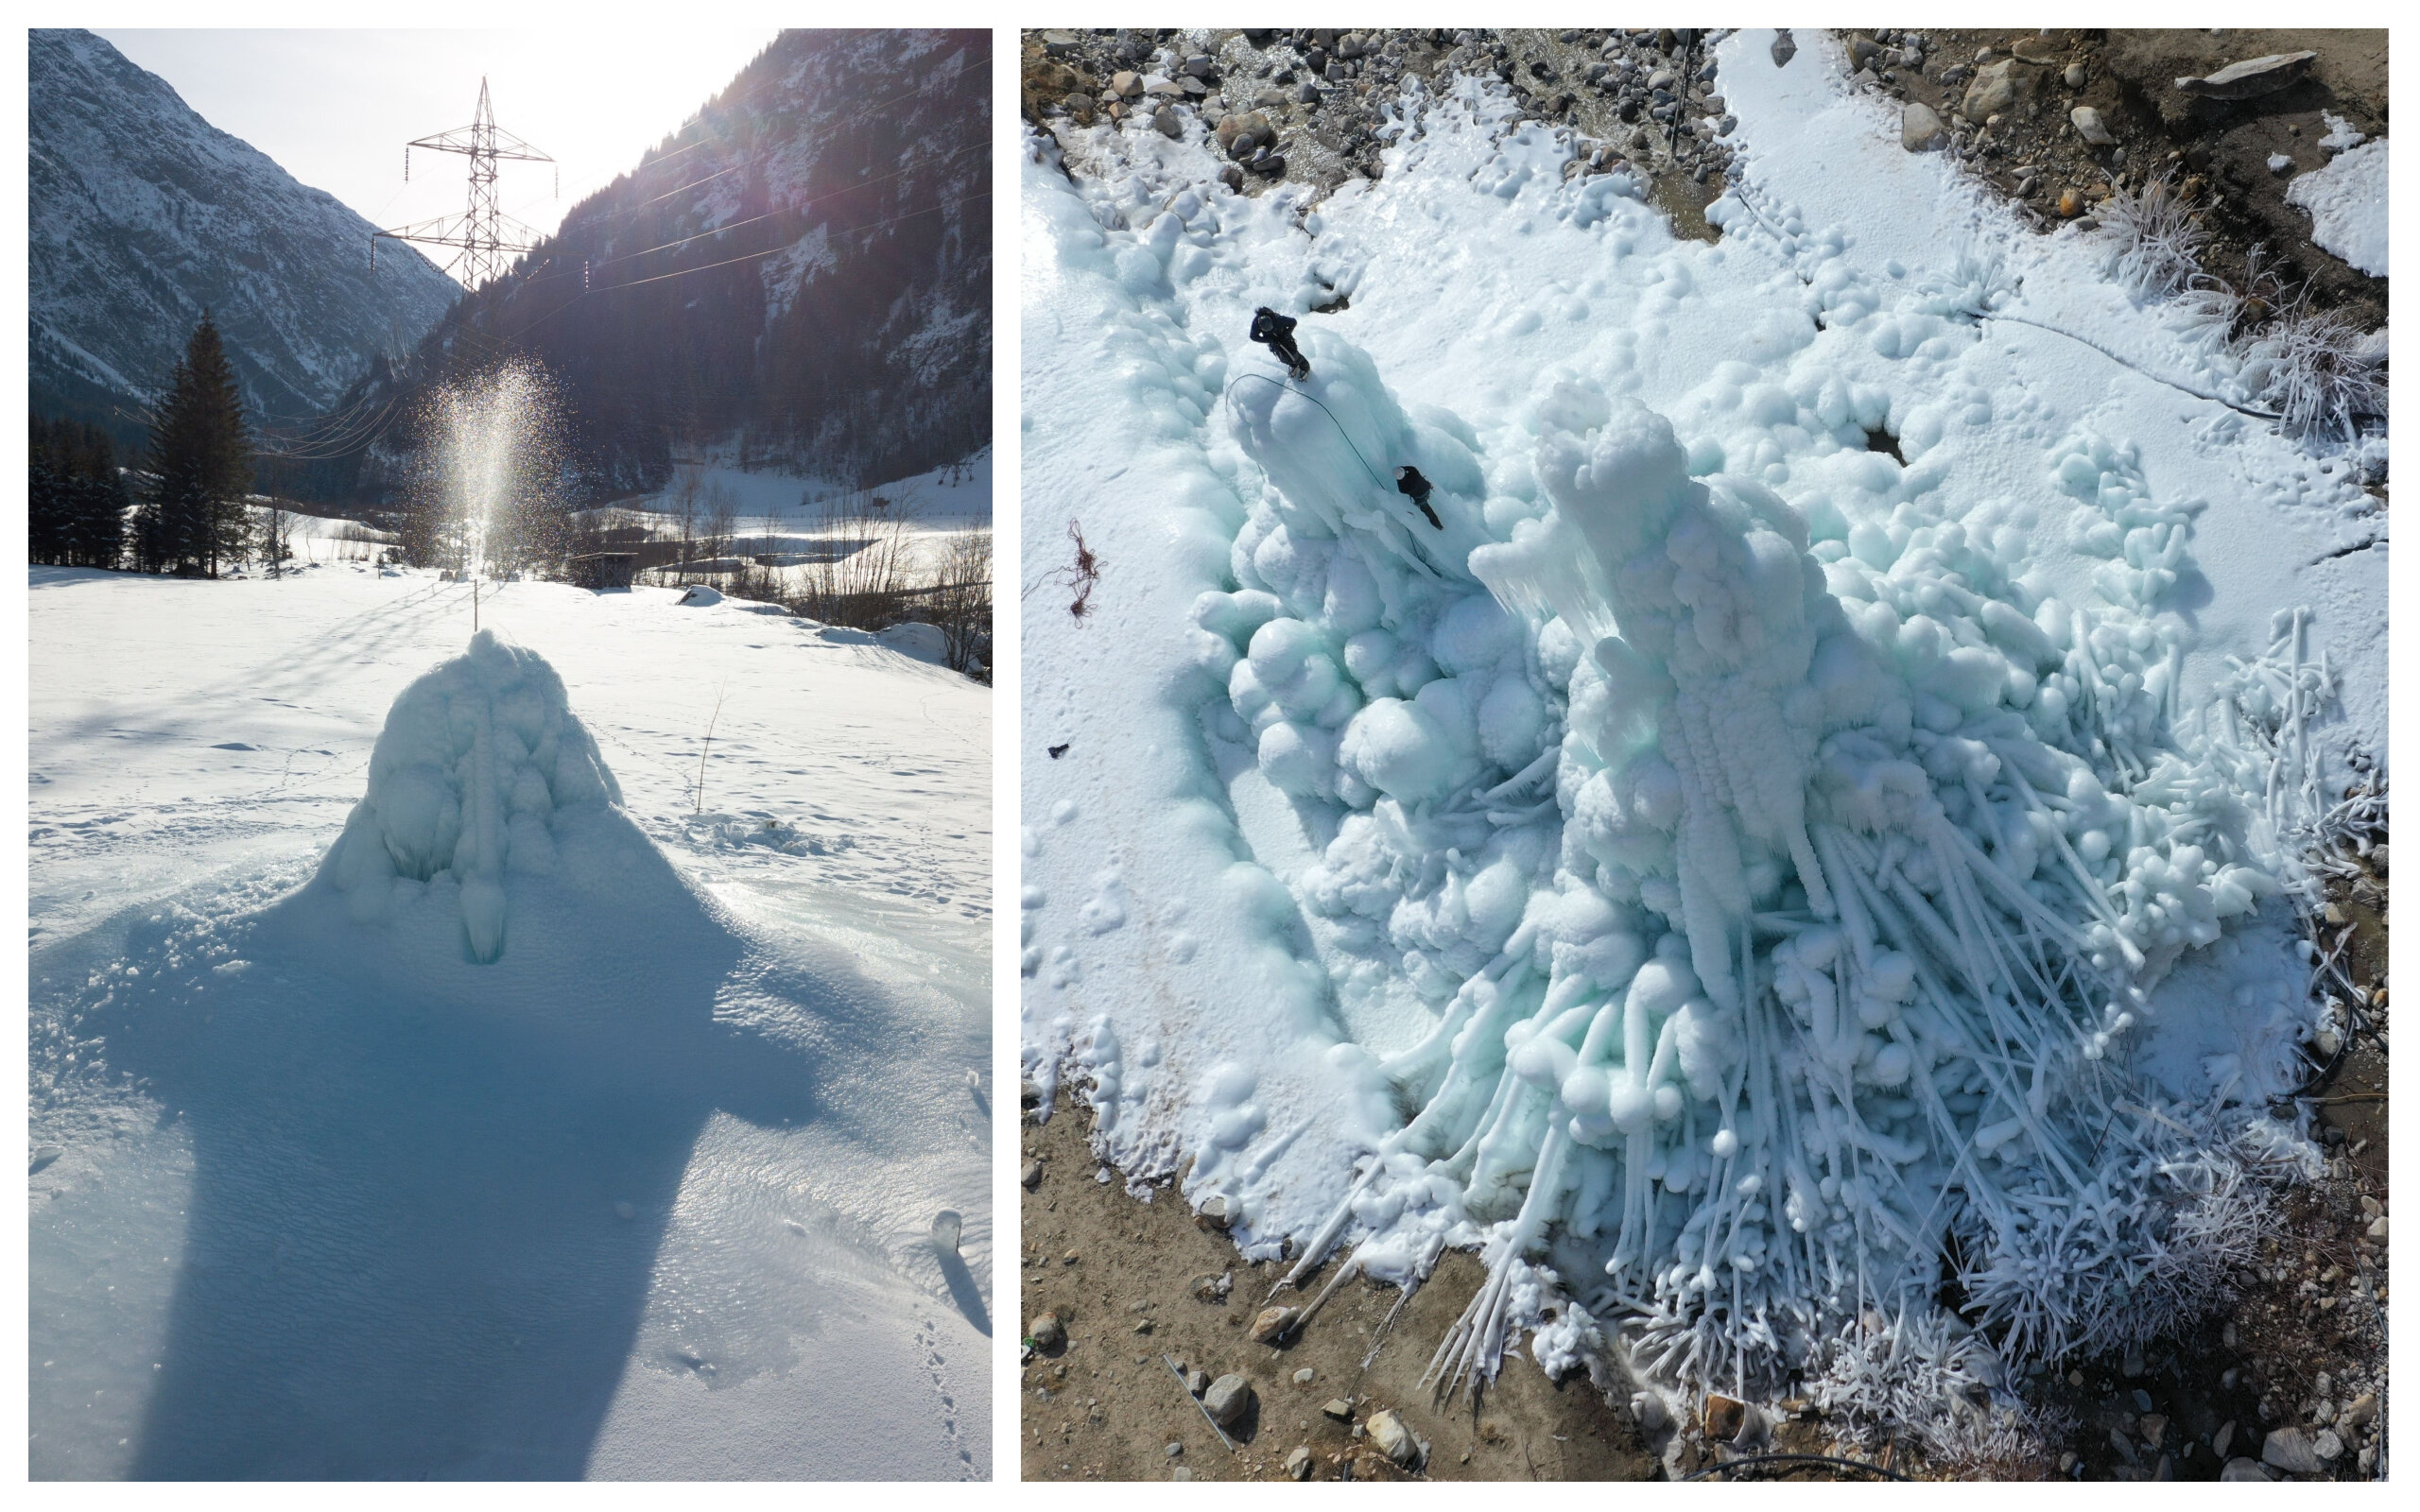
\includegraphics[width=12 cm]{Figures/Figure_2.jpg}
	\end{center}
	\caption{The Swiss and Indian AIR on January 9 and March 3, 2021 respectively. Picture credits: Daniel Buerki (left)
		and Thinles Norboo (right)}
	\label{fig:2AIR}
\end{figure}

The Gangles site (34.22 $\degree$N, 77.61 $\degree$E) is located around 20 km north of Leh city in the Ladakh
region, lying at 4025 $m$ a.s.l.. The mean annual temperature is $5.6 \, \degree C$, and the thermal range is
characterized by high seasonal variation. During January, the coldest month, the mean temperature drops to $-7.2
\, \degree C$. During August, the warmest month, the mean temperature rises to $17.5 \, \degree C$
\citep{Nusser_2012}. Because of the rain shadow effect of the Himalayan Range, mean annual precipitation in Leh
totals less than 100 mm, and there is high interannual variability. Whereas the average summer rainfall between
July and September reaches 37.5 mm, the average winter precipitation between January and March amounts to 27.3
mm and falls almost entirely as snow .  AIR were constructed here as part of the Icestupa Competition  by the
Himalayan Institute of Alternatives, Ladakh (HIAL). The fountain height of the AIR varied between 5 to 9\,$m$.

\subsection{Meteorological data}

Air temperature, relative humidity, wind speed, pressure, longwave, shortwave direct and diffuse radiation are
required to calculate the surface energy balance of an AIR (see Table \ref{tab:Observations}).

For the CH site, the primary weather data source was a Meteoswiss AWS located 184 m away . In addition, we used ERA5 reanalysis dataset \citep{era5} for filling data gaps and
adding the shortwave and longwave radiation data that were not measured directly.  The ERA5 reanalysis dataset
has a good correlation with sites in Switzerland \citep{Scherrer_2020}. The ERA5 grid point
chosen (46.64 $\degree$N, 8.25 $\degree$E) for the Swiss site was around 3.6 km away from the actual site. ERA5
variables (except incoming shortwave and longwave radiation) were fitted with the meteoswiss dataset via linear
regressions. The zero wind speed values recorded by the Meteoswiss AWS whenever snow accumulated on the
ultrasonic wind sensor were replaced using the ERA5 dataset.

For the IN site, two different weather data sources were used to log all the weather parameters required for the
model. Temperature, humidity, wind speed and pressure data was logged via a campbell weather station located 440
m away from the construction site. Shortwave radiation data was derived from another campbell weather station
located 15 km away. Unfortunately, precipitation was not logged. Since winter precipitation in Ladakh is less
than 30 mm \citep{Nusser_2012}, we can safely assume negligible precipitation and mostly clear skies. As a
consequence, the diffuse fraction of the global shortwave radiation was also assumed to be negligible .

\begin{table}
	\centering
	\caption{Summary of the weather and fountain observations. The weather measurements are shown using their
		mean ($\mu$) and standard deviation ($\sigma$) during the simulation duration as $\mu \pm \sigma$. }
	\label{tab:Observations}
	\begin{tabular}{@{}|lllllll|@{}}
		\toprule
		\textbf{}              & \textbf{Name}               & \textbf{Symbol} & \textbf{IN21} &
		\textbf{CH21}          & \textbf{CH20}               & \textbf{Units}                                                              \\ \midrule
		\multicolumn{1}{|l|}{\multirow{9}{*}{\rotatebox[origin=c]{90}{Weather}}}
		                       & Air temperature             & $T_a    $       & $0 \pm 7$     & $2 \pm 6$    & $2
		\pm 4$                 & $\degree C$                                                                                               \\
		\multicolumn{1}{|l|}{} & Relative humidity           & $RH     $       & $35 \pm 20$   & $79 \pm 18$  & $77
		\pm 17$                & \%                                                                                                        \\
		\multicolumn{1}{|l|}{} & Wind speed                  & $v_a        $   & $3 \pm 1$     & $2 \pm 2$    &
		$2 \pm 2$              & $m/s$                                                                                                     \\
		\multicolumn{1}{|l|}{} & Direct Shortwave            & $SW_{direct} $  & $246 \pm 333$ & $80 \pm 156$
		                       & $80 \pm 150$                & $W\,m^{-2}$                                                                 \\
		\multicolumn{1}{|l|}{} & Diffuse Shortwave           & $SW_{diffuse}$  & $0 \pm 0$     & $58 \pm 87$  & $51 \pm 74$  & $W\,m^{-2}$ \\
		\multicolumn{1}{|l|}{} & Incoming Longwave Radiation & $LW_{in}$       & $194 \pm 31$  & $239 \pm 35$ & $236 \pm 34$ & $W\,m^{-2}$ \\
		\multicolumn{1}{|l|}{} & Hourly Precipitation        & $ppt        $   & $0 \pm 0$     & $139 \pm
		457$                   & $95 \pm 404$                & $mm$                                                                        \\
		\multicolumn{1}{|l|}{} & Pressure                    & $p_a         $  & $623 \pm 3$   & $794 \pm 9$  &
		$798 \pm7$             & $hPa$                                                                                                     \\
		\multicolumn{1}{|l|}{} & Simulation Duration         & $h_{total} $    & 3673          & 4003
		                       & 1844                        & $hours$                                                                     \\
		\multicolumn{1}{|l|}{} & Simulation Start Date         &     & Jan 18 2021   & Nov 22 2020
		                       & Jan 3 2020                       &                                                                      \\\bottomrule
		\multicolumn{1}{|l|}{\multirow{4}{*}{\rotatebox[origin=c]{90}{Fountain}}}
		                       & Discharge rate             & $d_F     $      & $60$          & $7.5$        &
		$7.5$                  & $l/min$                                                                                                   \\
		\multicolumn{1}{|l|}{} & Runtime                     & $t_F $          & 829           & 2155
		                       & 1553                        & $hours$                                                                     \\
		\multicolumn{1}{|l|}{} & Spray radius                & $r_{F}$         & 10.8          & 6.9
		                       & 7.7                         & $m$                                                                         \\
		\multicolumn{1}{|l|}{} & Water temperature           & $T_{F}$         & 1             & 3
		                       & 3                           & $\degree C$                                                                 \\\midrule
	\end{tabular}
\end{table}


\subsection{Fountain observations}

We define the fountain used through four attributes, namely its spray radius, mean discharge quantity, discharge
runtime and water temperature as shown in Table \ref{tab:Observations}. Continuous measurement of the discharge
rate was unsuccessful in all the sites due to data logger malfunctions of the associated flowmeter. Instead the
discharge duration was first determined and then the available discharge measurement was used to determine the
average discharge quantity $d_F$ during these periods.  The spray radius $r_F$ was estimated from the mean AIR
circumference measured in the drone surveys during the fountain runtime.

The Swiss fountain discharge duration was extrapolated from just one fountain on and off event each. Even though
the Indian fountain was never manually switched off, there were many pipeline freezing events that interrupted
the discharge duration. Discharge rate was extrapolated to be the mean discharge $d_F$ except during these
pipeline freezing events.

\subsection{Drone surveys}

Several photogrammetric surveys using drones were conducted on the Swiss and Indian sites. The details of these
surveys and the methodology used to produce the corresponding outputs are explained in Appendix \ref{sec:uav} .
The digital elevation maps (DEMs) generated from the obtained imagery were analysed to document the radius,
surface area and volume of the ice structure. The number of surveys available for the IN21, CH21 and CH20 AIR
were 6, 8 and 2 respectively (see Table \ref{tab:uav}). The first drone flight was used to set the dome volume
($V_{dome}$) for model initialisation. The remaining surveys were used for model calibration and validation.
Since the Indian AIR was built on top of another ice structure (see Fig. \ref{fig:2AIR}), it had a much higher
dome volume compared to the other AIRs.  

\begin{table}
	\centering
	\caption{ Summary of the drone surveys}
	\label{tab:uav}
	\begin{tabular}{@{}|llllll|@{}}
		\toprule
		\textbf{}              & \textbf{No.} & \textbf{Date} & \textbf{Volume} & \textbf{Radius} & \textbf{Surface Area} \\ \midrule
		\multicolumn{1}{|l|}{\multirow{6}{*}{\rotatebox[origin=c]{90}{IN21}}}
		                       & 1            & Jan 18, 2021  & 103 $m^{3}$     & 9.1 $m$
		                       & 411 $m^{2}$                                                                      \\
		\multicolumn{1}{|l|}{} & 2            & Feb 27, 2021  & 580 $m^{3}$     & 10.2 $m$
		                       & 668 $m^{2}$                                                                      \\
		\multicolumn{1}{|l|}{} & 3            & Mar 3, 2021   & 626 $m^{3}$     & 10.3 $m$
		                       & 694 $m^{2}$                                                                      \\
		\multicolumn{1}{|l|}{} & 4            & Mar 15, 2021  & 692 $m^{3}$     & 10 $m$
		                       & 681 $m^{2}$                                                                      \\
		\multicolumn{1}{|l|}{} & 5            & Mar 26, 2021  & 582 $m^{3}$     & 10.2 $m$
		                       & 671 $m^{2}$                                                                      \\
		\multicolumn{1}{|l|}{} & 6            & Apr 3, 2021   & 620 $m^{3}$     & 10.1 $m$
		                       & 658 $m^{2}$
		\\\midrule
		\multicolumn{1}{|l|}{\multirow{8}{*}{\rotatebox[origin=c]{90}{CH21}}}
		                       & 1            & Nov 22, 2020  & 13 $m^{3}$      & 5.4 $m$
		                       & 136 $m^{2}$                                                                       \\
		\multicolumn{1}{|l|}{} & 2            & Dec 2, 2020   & 26 $m^{3}$      & 5.7 $m$
		                       & 118 $m^{2}$                                                                       \\
		\multicolumn{1}{|l|}{} & 3            & Dec 30, 2020  & 43 $m^{3}$      & 7.5 $m$
		                       & 189 $m^{2}$                                                                       \\
		\multicolumn{1}{|l|}{} & 4            & Jan 9, 2021   & 82 $m^{3}$      & 6.5 $m$
		                       & 150 $m^{2}$                                                                       \\
		\multicolumn{1}{|l|}{} & 5            & Mar 6, 2021   & 108 $m^{3}$     & 7.5 $m$
		                       & 183 $m^{2}$                                                                       \\
		\multicolumn{1}{|l|}{} & 6            & Apr 2, 2021   & 83 $m^{3}$      & 6.5 $m$
		                       & 150 $m^{2}$                                                                       \\
		\multicolumn{1}{|l|}{} & 7            & Apr 16, 2021  & 64 $m^{3}$      & 6.2 $m$
		                       & 134 $m^{2}$                                                                       \\
		\multicolumn{1}{|l|}{} & 8            & Apr 24, 2021  & 37 $m^{3}$      & 4.7 $m$
		                       & 80 $m^{2}$                                                                       \\
		\midrule
		\multicolumn{1}{|l|}{\multirow{2}{*}{\rotatebox[origin=c]{90}{CH20}}}
		                       & 1            & Jan 3, 2020   & 24 $m^{3}$      & 6.7 $m$
		                       & 170 $m^{2}$                                                                      \\
		\multicolumn{1}{|l|}{} & 2            & Jan 24, 2020  & 59 $m^{3}$      & 7.7 $m$
		                       & 228 $m^{2}$                                                                      \\
		\midrule
	\end{tabular}

\end{table}

\section{Model setup}

A bulk energy and mass balance model is used to calculate the amounts of ice, meltwater, water vapour and
wastewater of the AIR. In each hourly time step, the model uses the AIR surface area, energy balance and mass
balance calculations to estimate its ice volume, surface temperature and wastewater as shown in Fig.
\ref{fig:schema} .

\begin{figure}
	\begin{center}
		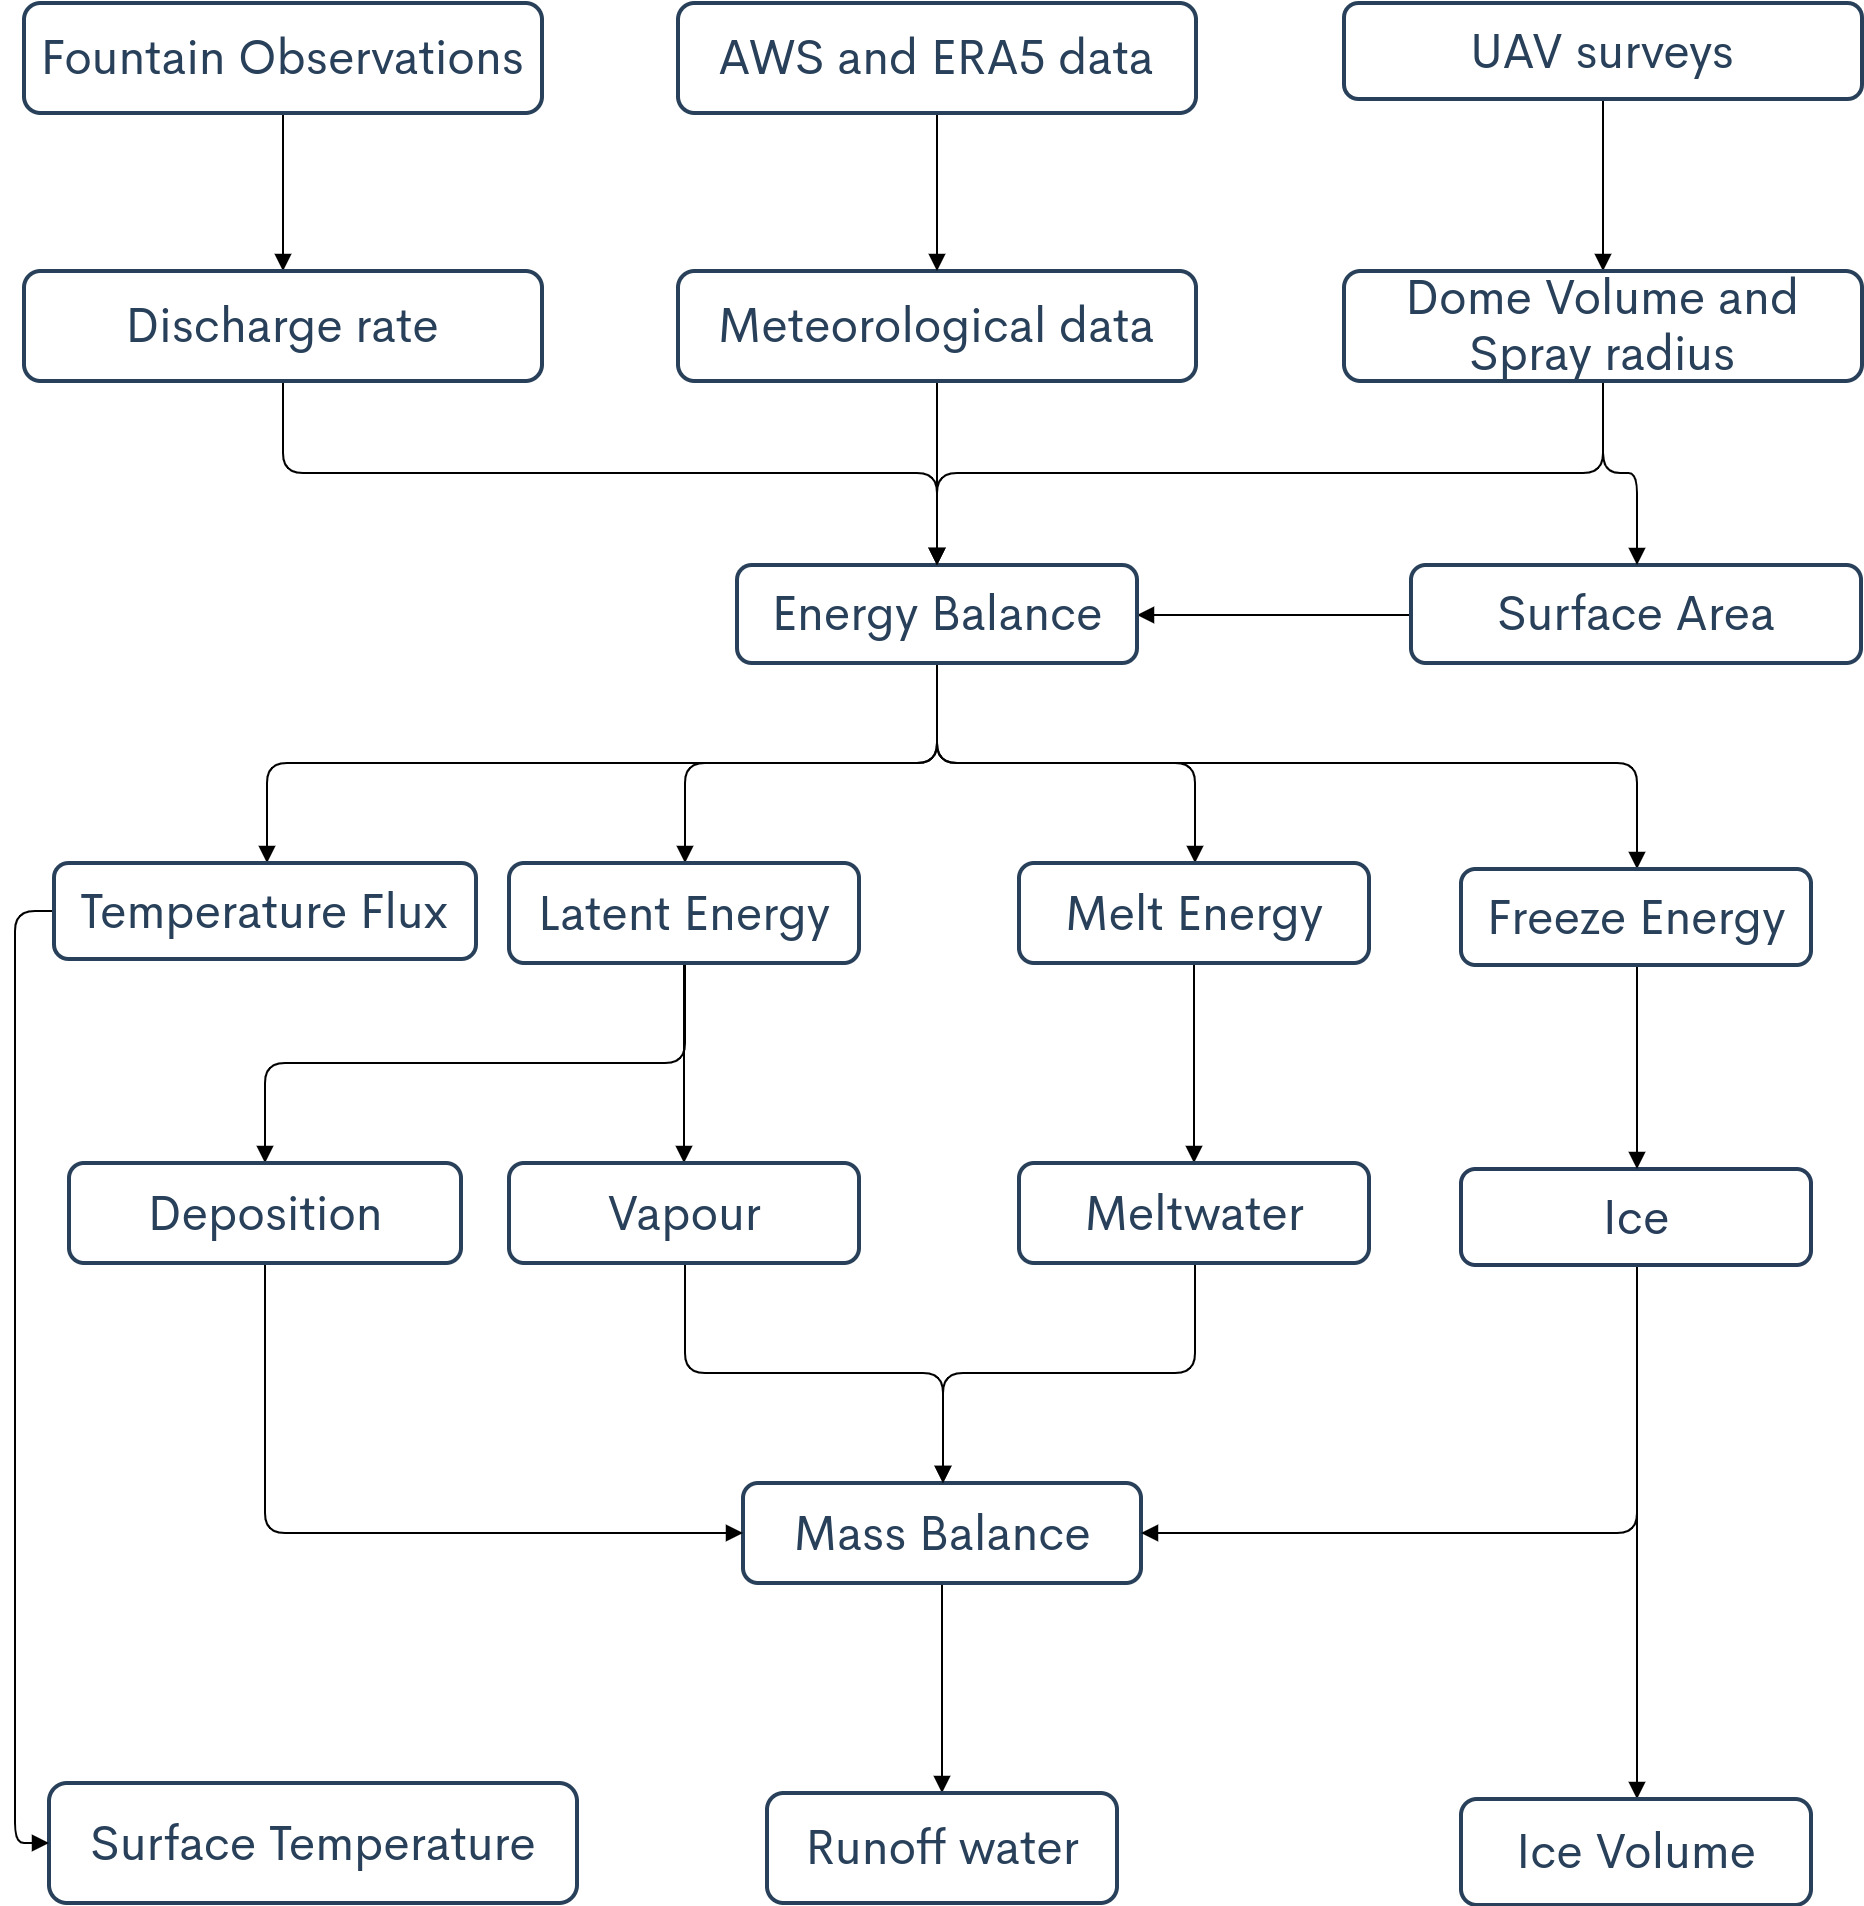
\includegraphics[width=10 cm]{Figures/Figure_3.jpg}
	\end{center}
	\caption{Model schematic showing the workflow used in the model at every time step. }
	\label{fig:schema}
\end{figure}

\subsection{Surface area calculation} \label{sec:shape}

The model assumes the AIR shape to be a cone and assigns the following shape attributes:

\begin{subequations}

	% \label{equations}
	\begin{align}
		\label{eq:A}
		A_{cone}^i & = \pi \cdot r_{cone}^i \cdot \sqrt{{(r_{cone}^i)}^2 + {(h_{cone}^i})^ 2} \\
		\label{eq:V}
		V_{cone}^i & = \pi/3 \cdot {(r_{cone}^i)}^2 \cdot h_{cone}^i                                         \\
		\label{eq:thickness}
		j_{cone}^i & =\frac{\Delta M_{ice}^i}{\rho_{water}* A_{cone}^i}
	\end{align}
\end{subequations}

where $i$ denotes the model time step, $r_{cone}^i$ is the radius; $h_{cone}^i$ is the height; $A_{cone}^i$ is
the surface area; $V_{cone}^i$ is the volume and $j_{cone}$ is the AIR surface normal thickness change as shown
in Fig. \ref{fig:shape}. $M_{ice}^i$ is the mass of the AIR and $\Delta M_{ice}^i = M_{ice}^{i-1} -
M_{ice}^{i-2}$. Henceforth, the equations used, display model time step superscript $i$ only if it is different
from the current time step.

AIR volume can also be expressed as:

\begin{equation} V_{cone} =\frac{M_{ice}} {\rho_{ice}} \label{eq:V1} \end{equation}

where $\rho_{ice}$ is the density of ice (917 $kg\, m^{-3}$). 

The initial radius of the AIR is assumed to be $r_F$. The initial height $h_0$ depends on the dome volume
$V_{dome}$ used to construct the AIR as follows:

\begin{equation}
	h_{0} =  \Delta x + \frac{3 \cdot V_{dome}}{\pi \cdot (r_F)^2 }
	\label{eq:h0}
\end{equation}

where $\Delta x$ is the surface layer thickness (defined in Section \ref{sec:energy})

During subsequent time steps, the dimensions of the AIR evolve assuming a uniform thickness change ($j_{cone}$)
across its surface area with an invariant slope $s_{cone} = \frac{h_{cone}}{r_{cone}}$ .  During these time
steps, the volume is parameterised using Eqn. \ref{eq:V} as:

\begin{equation} V_{cone} = \frac{\pi \cdot {(r_{cone})}^3
		\cdot s_{cone}}{3} \label{eq:V2} \end{equation}

We define the Icestupa boundary through its spray radius, i.e. we assume ice formation is negligible when $r_{cone} >
	r_{F}$. Combining Eqns. \ref{eq:V},  \ref{eq:V1}, \ref{eq:h0} and \ref{eq:V2}, the geometric evolution of the
Icestupa at each time step $i$ can be determined by considering the following rules:

\begin{equation} (r_{cone},\, h_{cone}) = \left\{ \begin{array}{ll} (r_F ,\, h_0)                                                                          & \textit{ if } i=0 \\
		(r_{cone}^{i-1},\, \frac{3 \cdot M_{ice}}{\pi \cdot \rho_{ice} \cdot {(r_{cone}^{i-1})}^2}) & \textit{ if }
		r_{cone}^{i-1} \geq r_{F} \textit{ and } \Delta M_{ice} > 0                                                     \\ (\frac{3 \cdot M_{ice}}{\pi \cdot \rho_{ice} \cdot s_{cone}})^{1/3} \cdot (1,\,  s_{cone}) &
		otherwise\end{array} \right.  \label{eq:A2} \end{equation}



\subsection{Energy balance calculation} \label{sec:energy}

\begin{figure}
	\begin{center}
		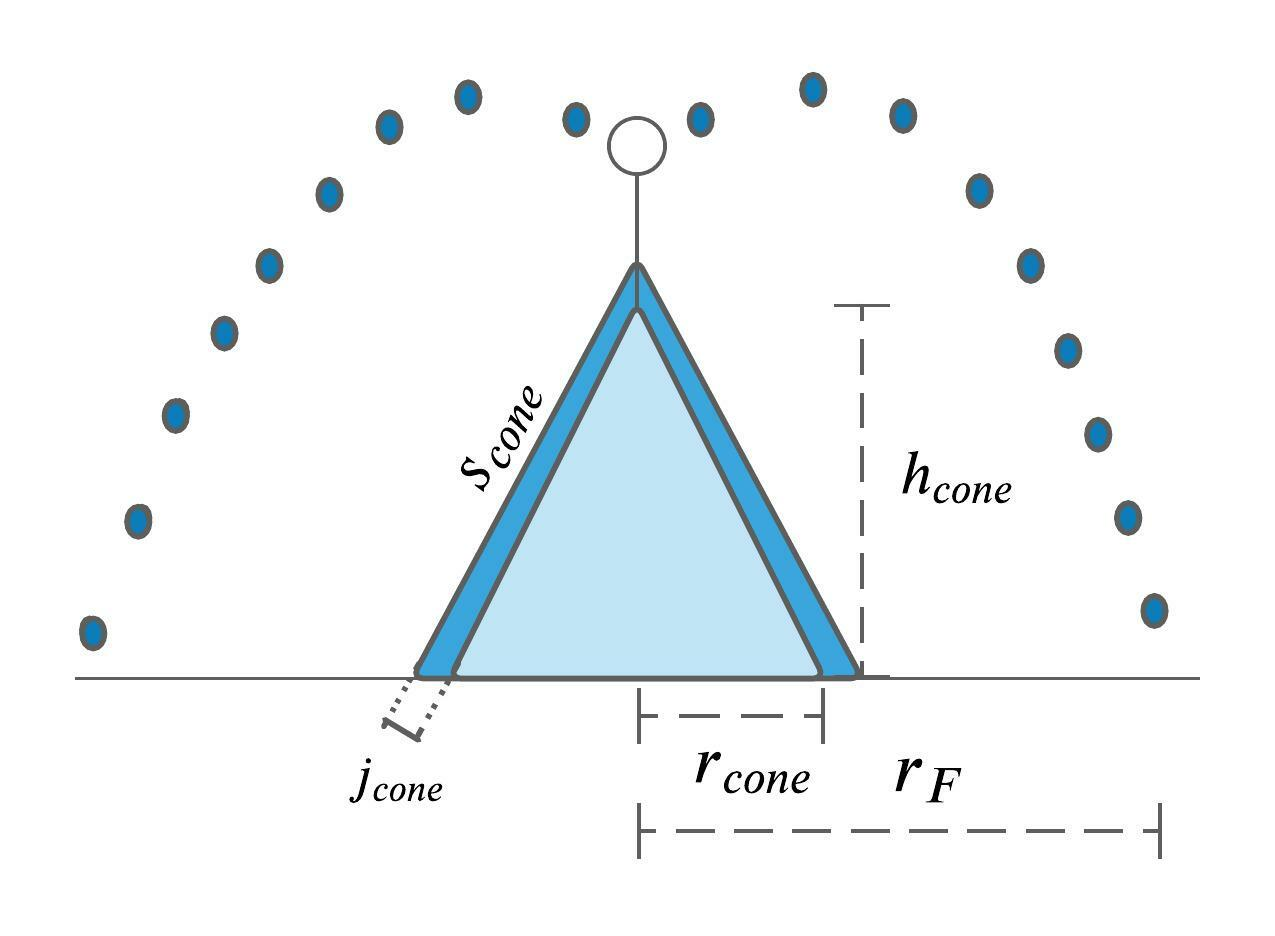
\includegraphics[width=10 cm]{Figures/Figure_4.jpeg}
	\end{center}
	\caption{Shape variables of the AIR. $r_{cone}$ is the radius, $h_{cone}$ is the height, $j_{cone}$ is the
		thickness change and $s_{cone}$ is the slope of the ice cone. $r_F$ is the spray radius of the fountain.}
	\label{fig:shape}
\end{figure}

We approximate the energy balance at the surface of an AIR by a one-dimensional description of energy fluxes
into and out of a (thin) layer with thickness $\Delta x$:

\begin{equation}
	\rho_{ice} \cdot c_{ice} \cdot \frac{\Delta T}{\Delta t} \cdot \Delta x = q_{SW} + q_{LW} + q_{L} + q_{S} + q_{F} + q_{G}
	\label{eqn:EB}
\end{equation}

Upward fluxes are positive and downward fluxes (into the ice surface) are negative. The first term is the energy change of the surface
layer, which can be translated into a phase change energy should phase changes occur; $q_{SW}$ is the net
shortwave radiation; $q_{LW}$ is the net longwave radiation; $q_{L}$ and $q_{S}$ are the turbulent latent and
sensible heat fluxes. $q_{F}$ represents the heat exchange of the fountain water droplets with the AIR ice
surface. $q_{G}$ represents ground heat flux between the AIR surface and its interior.

The energy flux acts upon the AIR surface layer, which has an upper and a lower boundary defined by the
atmosphere and the ice body of the AIR, respectively.  A sensitivity analysis was later performed
to understand the influence of this factor and decide its value. Here, we define the surface temperature
$T_{ice}$ to be the modelled average temperature of the Icestupa surface layer.

\subsubsection{Net Shortwave Radiation \texorpdfstring{$q_{SW}$}{Lg}}

The net shortwave radiation $q_{SW}$ is computed as follows:

\begin{equation} q_{SW} = (1- \alpha)\cdot (SW_{direct} \cdot f_{cone} + SW_{diffuse}) \label{eqn:SW} \end{equation}

where $SW_{direct}$ and $SW_{diffuse}$ are the direct and diffuse shortwave radiation, $\alpha$ is the
modelled albedo and $f_{cone}$ is the area fraction of the ice structure exposed to the direct shortwave
radiation.

The albedo varies depending on the water source that formed the current AIR surface layer. During the fountain
runtime, the albedo assumes a constant value corresponding to ice albedo. However, after the fountain is
switched off, the albedo can reset to snow albedo during snowfall events and then decay back to ice albedo. We
use the scheme described in \cite{OerlemansKnap_1998} to model this process. The scheme records the decay of
albedo with time after fresh snow is deposited on the surface. $\delta t$ records the number of time steps after
the last snowfall event. After snowfall, albedo changes over a time step, $\delta t$ , as

\begin{equation} \alpha=\alpha_{ice}+(\alpha_{snow}-\alpha_{ice}) \cdot e^{(-\delta t)/\tau} \label{eqn:a}
\end{equation}

where $\alpha_{ice}$ is the bare ice albedo value (0.25), $\alpha_{snow}$ is the fresh snow albedo value (0.85)
and $\tau$ is a decay rate (16 $days$), which determines how fast the albedo of the ageing snow recedes back to ice albedo.

The area fraction $f_{cone}$ of the ice structure exposed to the direct shortwave radiation depends on the shape
considered. Using the solar elevation angle $\theta_{sun}$, the solar beam can be considered to have a vertical
component, impinging on the horizontal surface (semicircular base of the AIR), and a horizontal component
impinging on the vertical cross section (a triangle). The solar elevation angle $\theta_{sun}$ used is modelled
using the parametrisation proposed by \cite{Woolf_1968}. Accordingly, $f_{cone}$ is determined as follows:

\begin{equation}
	\begin{split}
		f_{cone}& =\frac{(0.5 \cdot r_{cone} \cdot h_{cone}) \cdot cos \theta_{sun} +(\pi \cdot
			{(r_{cone})}^2/2) \cdot sin \theta_{sun} }{\pi \cdot r_{cone} \cdot ({(r_{cone})}^2+{(h_{cone})}^2)^{1/2}}\\
	\end{split}
	\label{eqn:f_{cone}}
\end{equation}

The diffuse shortwave radiation is assumed to impact the conical AIR surface uniformly.

\subsubsection{Net Longwave Radiation \texorpdfstring{$q_{LW}$}{Lg}} \label{sec:LW}

The net longwave radiation $q_{LW}$ is determined as follows:

\begin{equation}
	q_{LW}= LW_{in}-\sigma \cdot \epsilon_{ice} \cdot {(T_{ice}+ 273.15)}^4
	\label{eqn:LW}
\end{equation}

where $T_{ice}$ is the modelled surface temperature, both temperatures are given in [$\degree C$],
$\sigma=5.67\cdot10^{-8}\,Jm^{-2}s^{-1}K^{-4}$ is the Stefan-Boltzmann constant, $LW_{in}$ denotes the incoming
longwave radiation and $\epsilon_{ice}$ is the corresponding emissivity value for the Icestupa surface (0.97).

The incoming longwave radiation $LW_{in}$ for the Indian site, where no direct measurements were available, is
determined as follows:

\begin{equation}
	LW_{in}=\sigma \cdot (\epsilon_a \cdot {(T_a+ 273.15)}^4)
	\label{eqn:LWin}
\end{equation}

here $T_a$ represents the measured air temperature and $\epsilon_a$ denotes the atmospheric emissivity. We
approximate atmospheric emissivity $\epsilon_a$ using the equation suggested by \cite{Brutsaert_1982},
considering air temperature and vapor pressure (Eqn.  \ref{eqn:atm_e}). The vapor pressures over air and ice was
obtained using Eqn. \ref{eqn:vp}.  The expression defined in \cite{Brutsaert_1975} for clear skies (first term
in equation \ref{eqn:atm_e}) is extended with the correction for cloudy skies after \cite{Brutsaert_1982} as
follows:

\begin{equation}
	\epsilon_a=1.24 \cdot (\frac{p_{v,a}}{(T_a+273.15)})^{1/7}\cdot(1+0.22\cdot{cld}^2) \label{eqn:atm_e}
\end{equation}

with a cloudiness index $cld$, ranging from 0 for clear skies to 1 for complete overcast skies. For the Indian
site, we assume cloudiness to be negligible.

\subsubsection{Turbulent fluxes} \label{sec:Qs}

The turbulent sensible $q_{S}$ and latent heat $q_{L}$ fluxes are computed with the following expressions
proposed by \cite{Garratt_1992}:

\begin{equation}
	q_{S}=\mu_{cone}\cdot c_{a} \cdot \rho_{a} \cdot p_{a}/p_{0,a} \cdot \frac{\kappa^2 \cdot v_a \cdot
		(T_a-T_{ice})}{{(\ln{\frac{h_{AWS}}{z_{0}}})}^2}
	\label{eqn:qs}
\end{equation}

\begin{equation}
	q_{L}=\mu_{cone}\cdot 0.623 \cdot L_s \cdot \rho_{a}/p_{0,a} \cdot \frac{\kappa^2 \cdot
	v_a(p_{v,a}-p_{v,ice})}{{(\ln{\frac{h_{AWS}}{z_{0}}})}^2}
\end{equation}

where $h_{AWS}$ is the measurement height above the ground surface of the AWS (around $2\,m$ for all sites),
$v_a$ is the wind speed in [$m\,s^{-1}$], $c_a$ is the specific heat of air at constant pressure (1010 J
$kg^{-1} K^{-1}$), $\rho_{a}$ is the air density at standard sea level (1.29 $kg m^{-3}$), $p_{0,a}$ is the air
pressure at standard sea level (1013 $hPa$), $\kappa$ is the von Karman constant (0.4), $z_{0}$ is the surface
roughness (3 $mm$) and $L_s$ is the heat of sublimation (2848 $kJ\,kg^{-1}$).  The vapor pressures over air
($p_{v,a}$) and ice ($p_{v,ice}$) was obtained using the formulation given in \cite{WMO_2018} and
\cite{huang_2018} respectively  :

\begin{equation}
	\begin{split}
		p_{v,a}&=6.107 \cdot 10^{(7.5 \cdot T_a / (T_a + 237.3))} \cdot \frac{RH}{100}\\
		p_{v,ice}&=e^{(43.494 - \frac{6545.8}{T_{ice} + 278})}/(T_{ice} + 868)^2
	\end{split} \label{eqn:vp}
\end{equation}

where $p_{a}$ is the measured air pressure in [$hPa$].

The dimensionless parameter $\mu_{cone}$ is an exposure parameter that deals with the fact that AIR has a rough
appearance and forms an obstacle to the wind regime. This factor accounts for the larger turbulent fluxes due to
the roughness of the surface \citep{Oerlemans_2021}, and is a function of the AIR slope as follows:

\begin{equation}
	\mu_{cone} = 1 + \frac{s_{cone}}{2}
\end{equation}

A possible source of error is the fact that wind measurements from the horizontal plane at the AWS are used,
which might be different from those on a slope. However, without detailed datasets from the AIR surface, we
retain this assumption.

\subsubsection{Fountain discharge heat flux \texorpdfstring{$q_{F}$}{Lg} }

The fountain water, at temperature $T_F$, is assumed to cool to 0 $\degree C$. Thus, the heat flux caused by this
process is:

\begin{equation}
	q_{F} = \frac{ \Delta M_F \cdot c_{water} \cdot T_F}{\Delta t \cdot A_{cone}}
	\label{eqn:qF}
\end{equation}

with $c_{water}$ as the specific heat of water(4186 J $kg^{-1} K^{-1}$).

\subsubsection{Bulk Icestupa heat flux \texorpdfstring{$q_{G}$}{Lg}} \label{sec:Bulkflux}

The bulk Icestupa heat flux $q_{G}$ corresponds to the ground heat flux in normal soils and is caused by the
temperature gradient between the surface layer ($T_{ice}$) and the ice body ($T_{bulk}$). It is expressed by
using the heat conduction equation as follows:

\begin{equation} q_{G} = k_{ice} \cdot (T_{bulk}-T_{ice}^{i-1})/l_{cone} \label{eqn:qG}    \end{equation}

where $k_{ice}$ is the thermal conductivity of ice (2.123 $W\, m^{-1}\,K^{-1}$) , $T_{bulk}$ is the mean
temperature of the ice body within the Icestupa and $l_{cone}$ is the average distance of any point in the
surface to any other point in the ice body. $T_{bulk}$ is initialised as 0 $\degree C$ and later determined from
Eqn. \ref{eqn:qG} as follows:

\begin{equation} T_{bulk}^{i+1} = T_{bulk} - (q_{G} \cdot A \cdot \Delta t)/(M_{ice} \cdot c_{ice}) \end{equation}

Since AIRs typically have conical shapes with $r_{cone} > h_{cone}$, we assume that the center of mass of the cone
body is near the base of the fountain. Thus, the distance of every point in the AIR surface layer from the cone
body's center of mass is between $h_{cone}$ and $r_{cone}$. We calculate $q_{G}$ assuming $l_{cone} = (r_{cone} +
	h_{cone})/2$.

\subsubsection{Phase changes}

In this section, the numerical procedures to model phase changes at the surface layer are explained. Let
$T_{temp}$ be the calculated surface temperature. Even if the numerical heat transfer solution produces
temperatures which are $T_{temp}>0\, \degree C$, say from intense shortwave radiation, the ice temperature must
remain at $T_{temp} = 0\, \degree C$. The ‘‘excess’’ energy is used to drive the melting process. Moreover, the
energy input is used to melt the surface ice layer, and not to raise the surface temperature to some unphysical
value. Similarly, for freezing to occur, two conditions are required. Firstly, fountain water is present
($\Delta M_{F} > 0 $) and secondly the calculated temperature of the ice, $T_{temp}$, is below $0\, \degree C$.
Thus, depending on this surface temperature $T_{temp}$, the AIR can undergo further phase changes. So Eqn.
\ref{eqn:EB} can be rewritten as:

\begin{equation}
	q_{total}= q_{freeze/melt} + q_{T}
\end{equation}

where $q_{melt}$, $q_{freeze}$ and $q_{T}$ represent energy associated with melting, freezing and surface
temperature change processes respectively and the total energy available to be redistributed for these processes
is defined as $q_{total}=\rho_{ice} \cdot c_{ice} \cdot \frac{T_{temp}-T_{ice}}{\Delta t} \cdot \Delta x$.

We categorize every model time step as freezing or melting events. Freezing events can only occur, if fountain
water is available and $T_{temp}$ is below $0\,\degree C$. However, these two conditions are not sufficient as
the latent heat energy can only contribute to temperature fluctuations. Therefore, for preventing latent heat
energy from turning a melting event into a freezing event an additional condition namely, $(q_{total}-q_{L}) <
0$, is required.

\begin{equation}
	q_{freeze/melt} = \left\{ \begin{array}{ll}
		q_{freeze} & \textit{ if } \Delta M_{F} > 0 \textit{ and } T_{temp} < 0 \textit{ and }(q_{total}-q_{L}) < 0 \\
		q_{melt}   & \textit{ otherwise}
	\end{array} \right.
\end{equation}

During a freezing event, the AIR surface is assumed to warm to $0 \degree C$. The available energy
$(q_{total}-q_{L})$ is further augmented due to this change in surface temperature represented by the energy
flux:

$$q_{0} = \frac{\rho_{ice} \cdot \Delta x \cdot c_{ice} \cdot T_{ice}^{i-1}}{\Delta t}$$

The available fountain discharge may not be sufficient to utilize all the freezing energy. At such times, 
the additional freezing energy further cools down the surface temperature. Accordingly, the surface energy flux
distribution during a freezing event can be represented as:

\begin{equation}
	(q_{freeze}, q_{T}) = \left\{ \begin{array}{ll}
		(\frac{\Delta M_{F} \cdot L_f
		}{A_{cone} \cdot \Delta t}
		, q_{total}+\frac{\Delta M_{F} \cdot L_f
		}{A_{cone} \cdot \Delta t})          & \textit{ if  } \Delta M_{F} \textit{ insufficient }\\
		(q_{total}-q_{L}+q_{0}, q_{L}-q_{0}) & \textit{ otherwise }                                                                      \\
	\end{array} \right.
\end{equation}

If $T_{temp} > 0 \degree C$, then energy is reallocated from $q_{T}$ to $q_{melt}$ to maintain surface
temperature at melting point. The total energy flux distribution during a melting event can be represented as:

\begin{equation}
	(q_{melt}, q_{T}) = \left\{ \begin{array}{ll}
		(0, q_{total})                                                                                                                                                 & \textit{ if } T_{temp} < 0 \\
		(\frac{T_{temp} \cdot \rho_{ice} \cdot c_{ice} \cdot \Delta x}{\Delta t}, q_{total}-\frac{T_{temp} \cdot \rho_{ice} \cdot c_{ice} \cdot \Delta x}{\Delta t}  ) & \textit{ if } T_{temp} > 0
	\end{array} \right.
\end{equation}


\subsection{Mass balance calculation}

The mass balance equation for an AIR is represented as:

\begin{equation}
	\frac{\Delta M_{F} + \Delta M_{ppt} + \Delta M_{dep}}{\Delta t} = \frac{\Delta M_{ice} +\Delta M_{water} +
		\Delta M_{sub} + \Delta M_{waste}}{\Delta t}  \\
	\label{eq:MB}
\end{equation}

where $M_{F}$ is the cumulative mass of the fountain discharge; $M_{ppt}$ is the cumulative precipitation;  $M_{dep}$ is the cumulative
accumulation through water vapour deposition; $M_{ice}$ is the cumulative mass of ice; $M_{water}$ is the cumulative
mass of melt water; $M_{sub}$ represents the cumulative water vapor loss by sublimation and $M_{waste}$ represents the
fountain wastewater that did not interact with the AIR. The left hand side of equation \ref{eq:MB} represents the rate of
mass input and the right hand side represents the rate of mass output for an AIR.

Precipitation input is calculated as shown in equation \ref{eq:ppt} where $\rho_{w}$ is the density of water (1000
$kg\,m^{-3}$), $\Delta ppt/ \Delta t$ is the measured precipitation rate in [$m\,s^{-1}$] and $T_{ppt}$ is the temperature threshold
below which precipitation falls as snow. Here, snowfall events were identified using $T_{ppt}$ as $1 \degree C$. Snow
mass input is calculated by assuming a uniform deposition over the entire circular footprint of the AIR.

The latent heat flux is used to estimate either the evaporation and condensation processes or sublimation and deposition
processes as shown in equation \ref{eq:vap}. During time steps at which surface temperature is below 0 $\degree C$ only
sublimation and deposition can occur, but if the surface temperature reaches 0 $\degree C$, evaporation and condensation
can also occur. As the differentiation between evaporation and sublimation (and condensation and deposition) when the
air temperature reaches 0 $\degree C$ is challenging, we assume that negative (positive) latent heat fluxes correspond
only to sublimation (deposition), i.e. no evaporation (condensation) is calculated.

Since we have categorized every time step as a freezing or melting event, we can determine the ice and meltwater
generated using the associated energy fluxes as shown in equations \ref{eq:mwat} and \ref{eq:mcone}. Having calculated
all the other mass components the fountain wastewater generated every time step can be calculated using Eqn.
\ref{eq:MB}.

\begin{subequations}
	\begin{align}
		\frac{\Delta M_{F}}{\Delta t} & = \left\{ \begin{array}{ll} 0.06 \cdot d_F/\Delta t
			 & \textit{ if fountain is on} \\ 0 & \textit{ otherwise } \\\end{array} \right.                                             \\
		\label{eq:ppt}
		\frac{\Delta M_{ppt}}{\Delta t}                                    & = \left\{ \begin{array}{ll} \pi \cdot
        {(r_{cone})}^2 \cdot
			\rho_{w}\cdot \frac {\Delta ppt}{\Delta t} & \textit{ if } T_{a} < T_{ppt} \\ 0 & \textit{ if } T_{a} \geq T_{ppt} \\\end{array} \right.                                             \\
		\label{eq:vap}
		(\frac{\Delta M_{dep}}{\Delta t}, \frac{\Delta M_{sub}}{\Delta t}) & = \left\{ \begin{array}{ll} \frac{q_{L}
			\cdot A_{cone}}{L_s}\cdot (1,0)  & \textit{ if } q_{L} \geq 0 \\ \frac{q_{L}
			\cdot A_{cone}}{L_s}\cdot (0,-1) & \textit{ if } q_{L} < 0    \\\end{array} \right.                                             \\
		\label{eq:mwat}
		\frac{\Delta M_{water}}{\Delta t}                                  & = \frac{q_{melt} \cdot A_{cone} }{L_f}                                                   \\
	  \label{eq:m_freeze/melt}
    \frac{\Delta M_{freeze/melt}}{\Delta t} & = \frac{q_{freeze/melt} \cdot A_{cone} }{L_f} \\
		\label{eq:mcone}
		\frac{\Delta M_{ice}}{\Delta t}                                    & = \frac{q_{freeze}\cdot A_{cone} }{L_f} + \frac{\Delta M_{ppt}}{\Delta t} + \frac{\Delta
			M_{dep}}{\Delta t}- \frac{\Delta M_{sub}}{\Delta t}- \frac{\Delta M_{water}}{\Delta t}
	\end{align}
\end{subequations}

Considering AIRs as water reservoirs, their net water loss can be defined as:

\begin{equation} \textit{Net water losses} = \frac{M_{waste}+M_{sub}}{(M_F+M_{ppt}+M_{dep})} \cdot 100 \end{equation}

\subsection{Uncertainty Quantification}

The uncertainty in the model of estimating ice volumes are caused due to three sources, namely, model forcing
data, model hyperparameters and model parameters. Model forcing data can further be divided into weather and
fountain forcing data. Significant uncertainty exists in the weather forcing data, particularly for all the
radiation measurements ($SW_{direct}, SW_{diffuse}, LW_{in}$) since they were taken from ERA5 dataset or an AWS
far away from the construction sites. But we are not accounting for uncertainties related to meteorological
forcing data in this analysis. Uncertainty in the fountain forcing data arises due to only some fountain
parameters listed in Table \ref{tab:parameters}. Fountain runtime $t_F$ has no uncertainty for the Swiss AIRs
because no interruptions occured during the study period. However, significant uncertainty exists for the IN21
AIR , where the interruptions due to pipeline freezing events happened overnight but this was ignored in this
analysis. Fountain spray radius $r_F$ was measured using the drone survey and therefore also doesn't contribute
to model uncertainty. The choice of $d_F$ for both sites was just a best guess, based on few observations made
by the flowmeter. So we associate this parameter by a large uncertainty of $\pm \,50\, \%$. For the fountain
water temperature $T_F$, we assumed an upper bound of $3\, \degree C$ since it is unlikely for it to have been
beyond this range considering winter conditions at all the sites. The model structure introduces uncertainty
through the spatial and temporal hyperparameters $\Delta x$ and $\Delta t$. We fix the temporal resolution of
the model at hourly timesteps and only investigate the uncertainty caused by $\Delta x$ here. Since the surface
layer thickness for an AIR does not resemble to any parameter in the glaciological literature, we attribute a
wide range of values for it (from 1 cm to 10 cm). The model parameters are henceforth called as weather parameters to distinguish
them from the fountain forcing parameters. These were fixed within a range based on literature values (see Table
\ref{tab:parameters}). 

Now we are left with three sets of uncertain parameters namely, model hyperparameters $Q^M = \Delta x$, fountain
forcing parameters $Q^F = [d_F, T_F]$ and weather parameters $Q^W = [\epsilon_{ice}, z_0, \alpha_{ice},
\alpha_{snow}, T_{ppt}, \tau]$. Together, these 9 parameters cause a large uncertainty in the ice volume
estimates. In order to reduce this uncertainty, we perform a global sensitivity analysis with the net water loss
as our objective. The focus of this sensitivity analysis was not on the absolute sensitivity towards single
parameters, but rather to reduce the dimension of the parameter space. Therefore, the following discussion was
limited to two classes: parameters to which the model was sensitive ($S_{T_{j}} > 0.5$) and non-sensitive
($S_{T_{j}} \leq 0.5$). The methodology to determine $S_{T_{j}}$ is described in Appendix \ref{sec:uncertainpy}.

Later, the sensitive model parameters were calibrated based on the root mean squared error (RMSE) between the
drone surveys (see Table \ref{tab:uav}) and the model estimations of the ice volume. For this calibration
procedure, all the insensitive parameters were set to the median value of their respective ranges defined in
Table \ref{tab:parameters}. Then, the model uncertainty was quantified separately for the remaining parameters
in $Q^M, Q^F$ and $Q^W$. The sensitivity analysis and calibration were carried out with the drone surveys of CH21
and IN21 AIRs. 

For validation, the calibrated model was tested with two datasets namely, the expiry date of all AIRs and the
drone surveys of CH20 AIR. The expiry date signifies the time when all the ice completely disappeared and only
the dome volume remains.

\begin{table}[h!]
  \caption{Free parameters in the model categorised as constant, derived, model hyperparameters, weather and
  fountain forcing parameters with their respective values/ranges.}

	\label{tab:parameters}
	\begin{tabular}{@{}llllll@{}}
		\toprule
		\textbf{Constant Parameters}                       & \textbf{Symbol} & \textbf{Value} &
    \textbf{Unit} & \textbf{References} \\\midrule
    Van Karman constant & $\kappa$      & 0.4        &dimensionless & \citeauthor{CuffeyPaterson_2010}              \\
    Stefan Boltzmann constant & $\sigma$ & $\num{5.67 e-8} $& $W\, m^{-2}\, K^{-4}$ & \citeauthor{CuffeyPaterson_2010}\\
    Air pressure at sea level & $p_{0,a}$ & 1013 & $hPa$  & \citeauthor{MolgHardy_2004}\\
    Density of water & $\rho_{w}$ & 1000 & $kg\, m^{-3}$    & \citeauthor{CuffeyPaterson_2010}\\
    Density of ice & $\rho_{ice}$ & 917 & $kg\, m^{-3}$ & \citeauthor{CuffeyPaterson_2010}\\
    Density of air & $\rho_{a}$ &  1.29 & $kg\, m^{-3}$   & \citeauthor{MolgHardy_2004}\\
    Specific heat of water & $c_{w}$ & 4186 & $J\, kg^{-1}\,\degree C^{-1}$  & \citeauthor{CuffeyPaterson_2010}\\
    Specific heat of ice & $c_{ice}$ & 2097 & $J\, kg^{-1}\,\degree C^{-1}$ & \citeauthor{CuffeyPaterson_2010}\\
    Specific heat of air & $c_{a}$ & 1010 & $J\, kg^{-1}\,\degree C^{-1}$ & \citeauthor{MolgHardy_2004}\\
    Thermal conductivity of ice & $k_{ice}$ & 2.123  & $W\, m^{-1}\, K^{-1}$ & \citeauthor{Bonales_2017} \\
    Latent Heat of Sublimation & $L_{s}$ & \num{2.848e6}  & $J\, kg^{-1}$ &   \citeauthor{CuffeyPaterson_2010}\\
    Latent Heat of Fusion & $L_{f}$ & \num{3.34e5} & $J\, kg^{-1}$ & \citeauthor{CuffeyPaterson_2010}\\
    Gravitational acceleration & $g$ & 9.81 & $m\, s^{-2}$ &\citeauthor{CuffeyPaterson_2010}\\\midrule
    % Weather station height & $h_{AWS}$ & 2 & $m$ & assumed \\\midrule
		\textbf{Derived Parameters} & \textbf{Symbol} & \textbf{} & \textbf{Unit} & \textbf{Section} \\\midrule
    Atmospheric emissivity & $\epsilon_{a}$ & & dimensionless    & \ref{sec:LW}\\
    Cloudiness & $cld$ &  & dimensionless  & assumed\\
    Vapour pressure over air & $p_{v,a}$ &  & $hPa$  & \ref{sec:Qs}\\
    Vapour pressure over ice & $p_{v,ice}$ &  & $hPa$ & \ref{sec:Qs}\\
    Radius of AIR & $r_{cone}$ &  & $m$ & \ref{sec:shape}\\
    Height of AIR & $h_{cone}$ &  & $m$ & \ref{sec:shape}\\
    Slope of AIR  & $s_{cone}$ &  & dimensionless & \ref{sec:shape}\\
    Thickness change of AIR  & $j_{cone}$ &  & $m$  & \ref{sec:shape}\\
    Ice body and surface distance & $l_{cone}$ &  & $m$  & \ref{sec:Bulkflux}\\
\midrule
		\textbf{Model Hyperparameters} & \textbf{Symbol} & \textbf{Range} & \textbf{Unit} & \textbf{References} \\\midrule
    % Surface Area correction factor      & $A_{corr}$            & $[1,2]$            & dimensionless       & assumed       \\
    Timestep                            & $\Delta t$            & $3600$           & $s$ & assumed \\
    Surface layer thickness             & $\Delta x$            & $[\num{1e-3},\num{1e-1}]$           & $m$ & assumed
    \\\midrule
		\textbf{Weather Parameters} & \textbf{Symbol} & \textbf{Range} & \textbf{Unit} & \textbf{References} \\\midrule
    Ice Emissivity                      & $\epsilon_{ice}$      & $[0.95,0.99]$         & dimensionless & \citeauthor{HORI2006486}             \\
    Surface Roughness                   & $z_0$                 & $[\num{1e-3},\num{5e-3}]$            & $m$  & \citeauthor{BrockWillisSharp_2006}       \\
    Ice Albedo                          & $\alpha_{ice}$        & $[0.15,0.35]$         & dimensionless  &
    \citeauthor{steiner_2015};            \\
    & &    &  & \citeauthor{ZollesMaussion_2019}      \\
    Snow Albedo                         & $\alpha_{snow}$       & $[0.8,0.9]$        & dimensionless  & \citeauthor{ZollesMaussion_2019}              \\
    Precipitation Temperature threshold & $T_{ppt}$             & $[0,2]$            & $\degree C$& \citeauthor{Zhou_2010}  \\
    Albedo Decay Rate                   & $\tau$                & $[10,22]$           & $days$ &
    \citeauthor{Schmidt_2017};      \\
    & &    &  & \citeauthor{OerlemansKnap_1998}      \\\midrule
		\textbf{Fountain Forcing Parameters} & \textbf{Symbol} & \textbf{Range} & \textbf{Unit} & \textbf{References} \\\midrule
    Discharge rate & $d_{F}$             & $\pm 50 \%$            & $l/min$& assumed  \\
    Water temperature & $T_{F}$             & $[0,3]$            & $\degree C$  & assumed  \\
    Spray radius & $r_{F}$             &             & $m$& measured \\
    Runtime & $t_{F}$             &             &  $hours$ & measured \\\bottomrule
	\end{tabular}
\end{table}

\section{Results}

\begin{figure}
	\begin{center}
		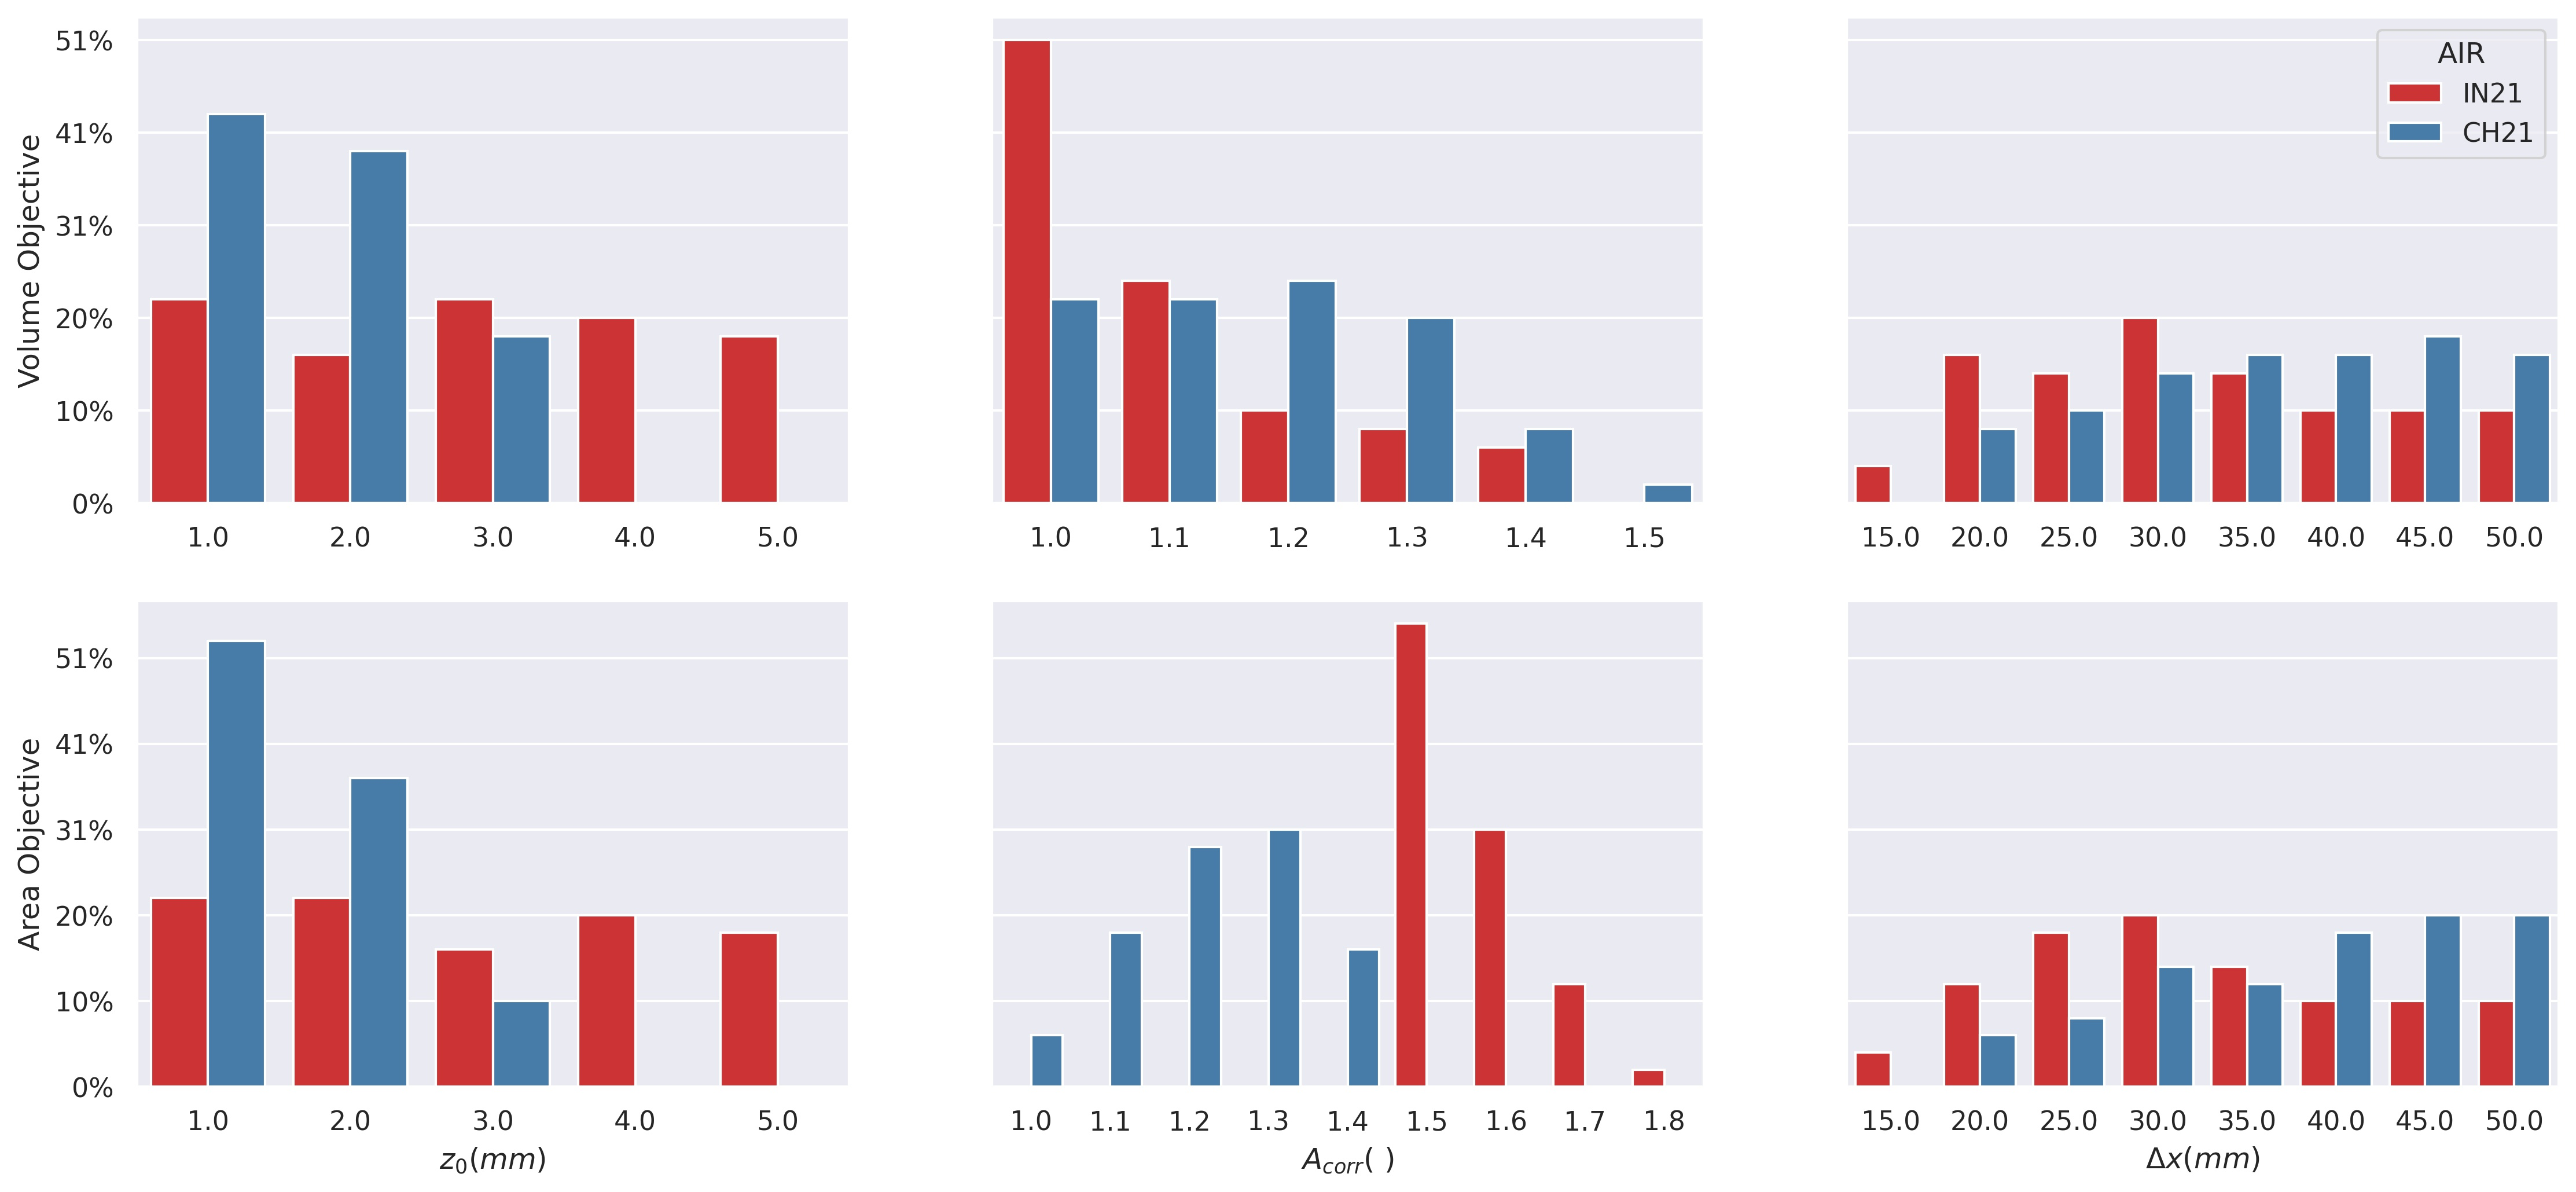
\includegraphics[width=\linewidth]{Figures/Figure_5.jpg}
	\end{center}
  \caption{(a) Total-order sensitivities of all the uncertain parameters of the model with net water loss as the
  objective. (b) The calibration of the sensitive parameter, $\Delta x$ with the RMSE between the drone and
model estimates of the ice volume. The dots denote the optimum values. The estimates from the Swiss and Indian
AIRs are denoted with blue and red colors respectively. }

	\label{fig:param_hist}
\end{figure}


\subsection{Calibration of sensitive parameters}

The total-order sensitivities of all the 9 parameters with respect to the net water loss objective are shown in
Fig. \ref{fig:param_hist} (a) . In total, global sensitivity analysis required 1432 model runs to determine these
sensitivities for each site. The only sensitive parameter ($S_{T_{j}} > 0.5$) for both the AIRs was the surface
layer thickness. The RMSE between the drone surveys and the model ice volume estimates for different surface
layer thickness are shown in Fig. \ref{fig:param_hist} (b). The optimum value of $\Delta x$ was found to be 45
$mm$ and 65 $mm$ with an RMSE of 9 $m^3$ and 30 $m^3$ for CH21 and IN21 AIRs respectively.


\subsection{Weather and fountain forcing uncertainty quantification}

The uncertainty in the ice volume estimates caused by the insensitive weather and fountain parameters are shown
in Fig. \ref{fig:results}. The ranges highlighted represent the $90\,\%$ prediction interval (defined in Appendix
\ref{sec:uncertainpy}) of the ice volume estimates. Weather uncertainty determination required 422 simulations
whereas fountain uncertainty determination required 32 simulations.

Weather uncertainty for IN21 was low compared to the other AIRs since precipitation and the associated variation
in albedo was negligible. This was expected since 4 out of the 5 insensitive weather parameters were part of the
albedo module. The remaining parameter, ice emissivity, caused the most variance in the ice volume estimate
among all the insensitive parameters ($S_{T_{\epsilon_{ice}}} = 0.7$).

Fountain forcing uncertainty for all the AIRs was high illustrating the importance of quantifying the fountain parameters for
a confident ice volume estimation. Among the 2 fountain parameters, ice volume variation was caused predominantly
by the uncertainty in the fountain's water temperature ($S_{T_{T_F}} = 0.8$).

\begin{figure}
	\begin{center}
		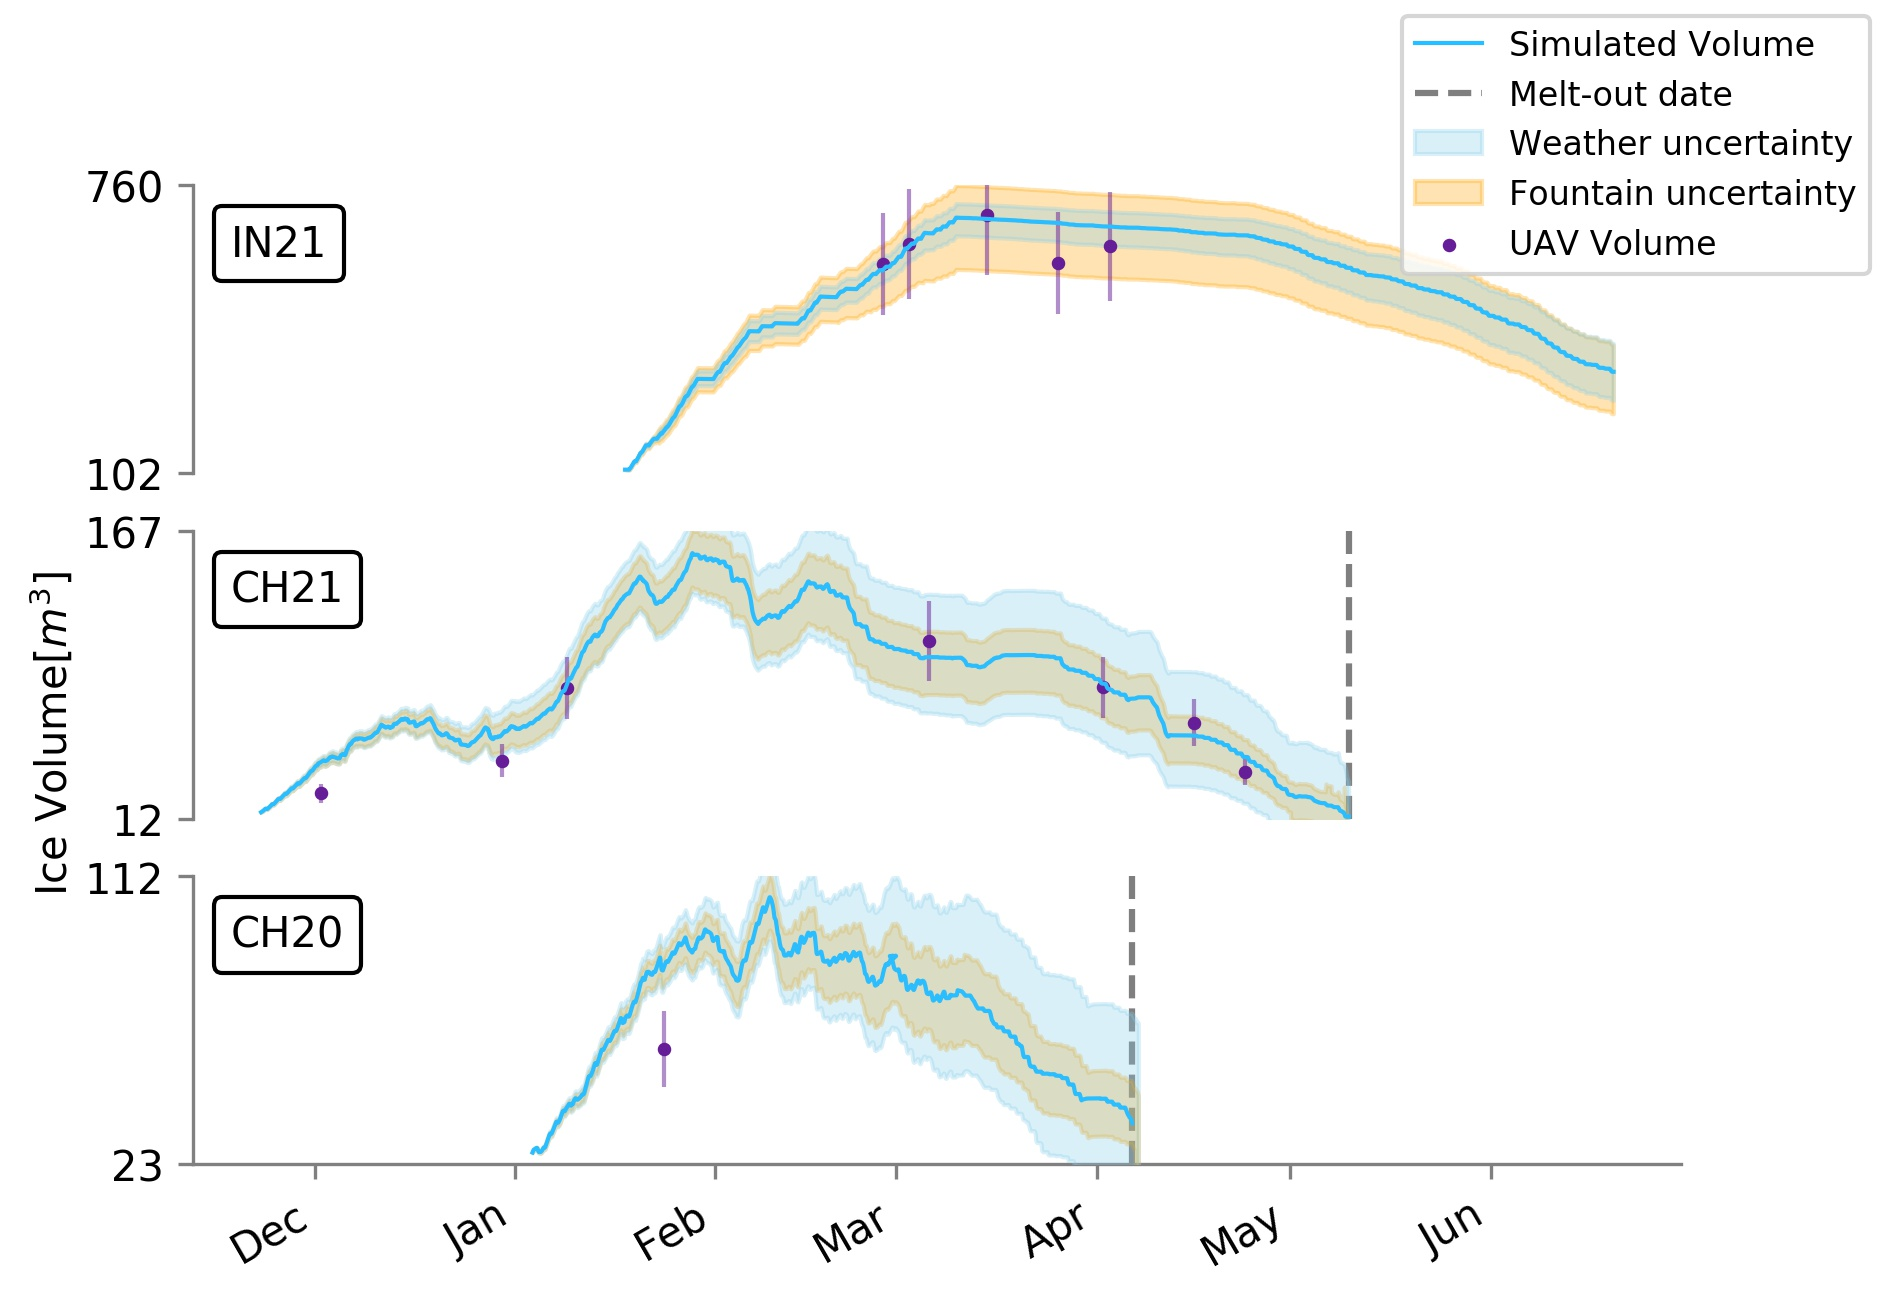
\includegraphics[width=\linewidth]{Figures/Figure_6.jpg}
	\end{center}
	\caption{Simulated ice volume during the lifetime of the AIRs (blue curve). The shaded regions (light blue and
		orange) represent the 90\% prediction interval of the AIR ice volume caused by the variations in weather and
    the fountain parameters, respectively. Violet points indicate the drone ice volume observations.  The grey
  dashed line represents the observed expiry date for each AIR.  }
	\label{fig:results}
\end{figure}

\subsection{Validation}

Model performance can be judged based on the ice volume left on the expiry date of all AIRs and the drone
surveys of the CH20 AIR. In the case of CH21 AIR no ice volume was left whereas for CH20 AIR ice volume of 12
$m^3$ was left on the expiry date. For the IN21 AIR, the determination of the expiry date was not possible. In
reality, the IN21 AIR was found to have disintegrated into several ice blocks on 20th June, 2021. There was just
one observation of the CH20 AIR volume (see Table \ref{tab:uav}). The RMSE of that observation with the modelled
volume was $19\, m^3$ which is 18 \% of the max ice volume of CH20 AIR.

\subsection{AIR ice volume estimates}

Since this model used a surface energy balance model commonly applied on glaciers, we analyse the AIR temporal
and spatial variation similar to how it is done for a glacier. Particularly, we used the AIR surface normal
thickness change ($j_{cone}$) as a measure to quantify the location influence. Note that $j_{cone}$ is similar
to the "specific mass balance" of a glacier with units $m \, w.\, e.$. Similarly, we divided the simulation duration
of the AIR into accumulation and ablation periods. The accumulation (ablation) period ends (starts) at the last
fountain discharge event. The thickness change during the accumulation and ablation period was referred to as
thickness growth and decay respectively.

The construction decisions responsible for the observed magnitude and variance of the ice volume estimates can
be categorised based on the fountain used and the location selected. According to Eqn.  \ref{eq:m_freeze/melt},
the freezing/melting rate of the AIRs can be decomposed to the corresponding freezing/melting energy and the
surface area. The construction location chosen determines the thickness growth/decay through the
freezing/melting energy flux and the fountain determines the surface area through its spray radius.

The influence of location can be further comprehended, if we analyse the daily surface normal thickness change
together with the corresponding energy fluxes. Fig. \ref{fig:MEB} shows the daily thickness and energy balance
components calculated with the calibrated surface layer thickness for the first and last 20 days for each AIR. The two time
periods selected were characteristic of the accumulation and ablation period, respectively. A strong variability
was evident between the accumulation and ablation periods and between the CH21 and the IN21 AIR.

The daily mean thickness change of the Indian location was positive ($3\, mm \,w.e.$) with a daily mean growth
of $31\, mm \,w.e.$ and a mean decay of $11\, mm \,w.e.$. In the Swiss location, the daily mean
thickness change was negative ($-4\, mm \,w.e.$) with a daily mean thickness growth of $8\, mm \,w.e.$ and a
mean decay of $18\, mm \,w.e.$. The difference in magnitude between the growth and the decay corresponds to the
difference between the freezing and the melting energy balance components. For the Indian site, $q_{freeze}$
accounted for 73 \%, $q_{melt}$ accounted for 23 \% and $q_{T}$ just 4 \% of overall energy turnover. The energy
turnover is calculated as the sum of energy fluxes in absolute values. For the Swiss site, $q_{freeze}$
accounted for 37 \%, $q_{melt}$ accounted for 61 \%  and $q_{T}$ just 2 \% of overall energy turnover. The
freezing events occurred for 19\% and 34\% of the simulation duration (see Table \ref{tab:Observations}) for the
Indian and Swiss site respectively. The accumulation period is characteristic of these freezing events and
ablation period is characteristic of the melting events. We compare the energy turnover of different energy
fluxes between these two periods to quantify the influence of different surface processes.

\begin{table}
	\centering
  \caption{ Contribution of the energy balance components (EBC) to the total energy turnover (the sum of energy
    fluxes in absolute values) during the accumulation and ablation periods with their daily mean ($\mu$) and
  standard deviation ($\sigma$) for each site. The positive/negative sign is indicative of the upward/downward
direction of the mean energy flux during the respective period.}

	\label{tab:turnover}
	\begin{tabular}{@{}|lllll|@{}}
		\toprule
		\textbf{}              & \textbf{EBC} & \textbf{Accumulation} & \textbf{Ablation} & \textbf{$\mu \pm \sigma
			$}                                                                                                             \\ \midrule
		\multicolumn{1}{|l|}{\multirow{6}{*}{\rotatebox[origin=c]{90}{IN21}}}
		                       & $q_{SW}$     & 16 \%                  & 25 \%             & $ 26 \pm 43 \, W\,m^{-2}$  \\
		\multicolumn{1}{|l|}{} & $q_{LW} $    & -43 \%                & -25 \%            & $ -80\pm 34 \, W\,m^{-2}$  \\
		\multicolumn{1}{|l|}{} & $q_{S}  $    & 13 \%                 & 30 \%             & $ 96 \pm140 \, W\,m^{-2}$  \\
		\multicolumn{1}{|l|}{} & $q_{L}  $    & -24 \%                & -20 \%            & $ -52 \pm 74 \, W\,m^{-2}$ \\
		\multicolumn{1}{|l|}{} & $q_{F}  $    & 4 \%                  & 0 \%              & $ 2 \pm 3 \, W\,m^{-2}$    \\
		\multicolumn{1}{|l|}{} & $q_{G}   $   & 0\%                   & 0 \%              & $ 0 \pm 2 \, W\,m^{-2}$    \\\midrule
		\multicolumn{1}{|l|}{\multirow{6}{*}{\rotatebox[origin=c]{90}{CH21}}}
		                       & $q_{SW} $    & 21 \%                 & 23 \%             & $ 37 \pm 56 \, W\,m^{-2}$  \\
		\multicolumn{1}{|l|}{} & $q_{LW} $    & -41 \%                & -29 \%            & $ -57 \pm 33 \, W\,m^{-2}$ \\
		\multicolumn{1}{|l|}{} & $q_{S}  $    & 23 \%                 & 39 \%             & $ 36 \pm 74 \, W\,m^{-2}$  \\
		\multicolumn{1}{|l|}{} & $q_{L}  $    & -11 \%                 &10 \%              & $ -2 \pm 31 \, W\,m^{-2}$  \\
		\multicolumn{1}{|l|}{} & $q_{F}  $    & 3 \%                  & 0 \%              & $ 5 \pm 4 \, W\,m^{-2}$    \\
		\multicolumn{1}{|l|}{} & $q_{G}   $   & 0 \%                  & 0 \%              & $ 0 \pm 1 \, W\,m^{-2}$    \\\bottomrule
	\end{tabular}
\end{table}

To understand the overall impact of the radiation fluxes (longwave and shortwave) and the turbulent fluxes
(sensible and latent) on the freezing and melting energies, we sum their respective energy turnover taking into
account the sign of their mean energy during the accumulation/ablation period (see Table \ref{tab:turnover}). A
negative sign indicates that the corresponding energy flux increased/decreased the freezing/melting energy
respectively. Note that all the energy fluxes maintain the same sign for both the accumulation and ablation
periods for the Indian location but the latent heat changes sign for the Swiss location. The radiation fluxes
contributed -27 \% and 0 \% to the freezing and melting energies for the Indian location and -20 \% and -6 \%
to the Swiss location respectively.  Similarly, the turbulent fluxes at the Indian location contribute -11 \% and
10 \% and at the Swiss location contribute 12 \% and 49\%  respectively. So the AIR thickness growth was
driven by the net radiation fluxes and the AIR thickness decay was driven by the net turbulent fluxes.

\begin{figure}
	\begin{center}
		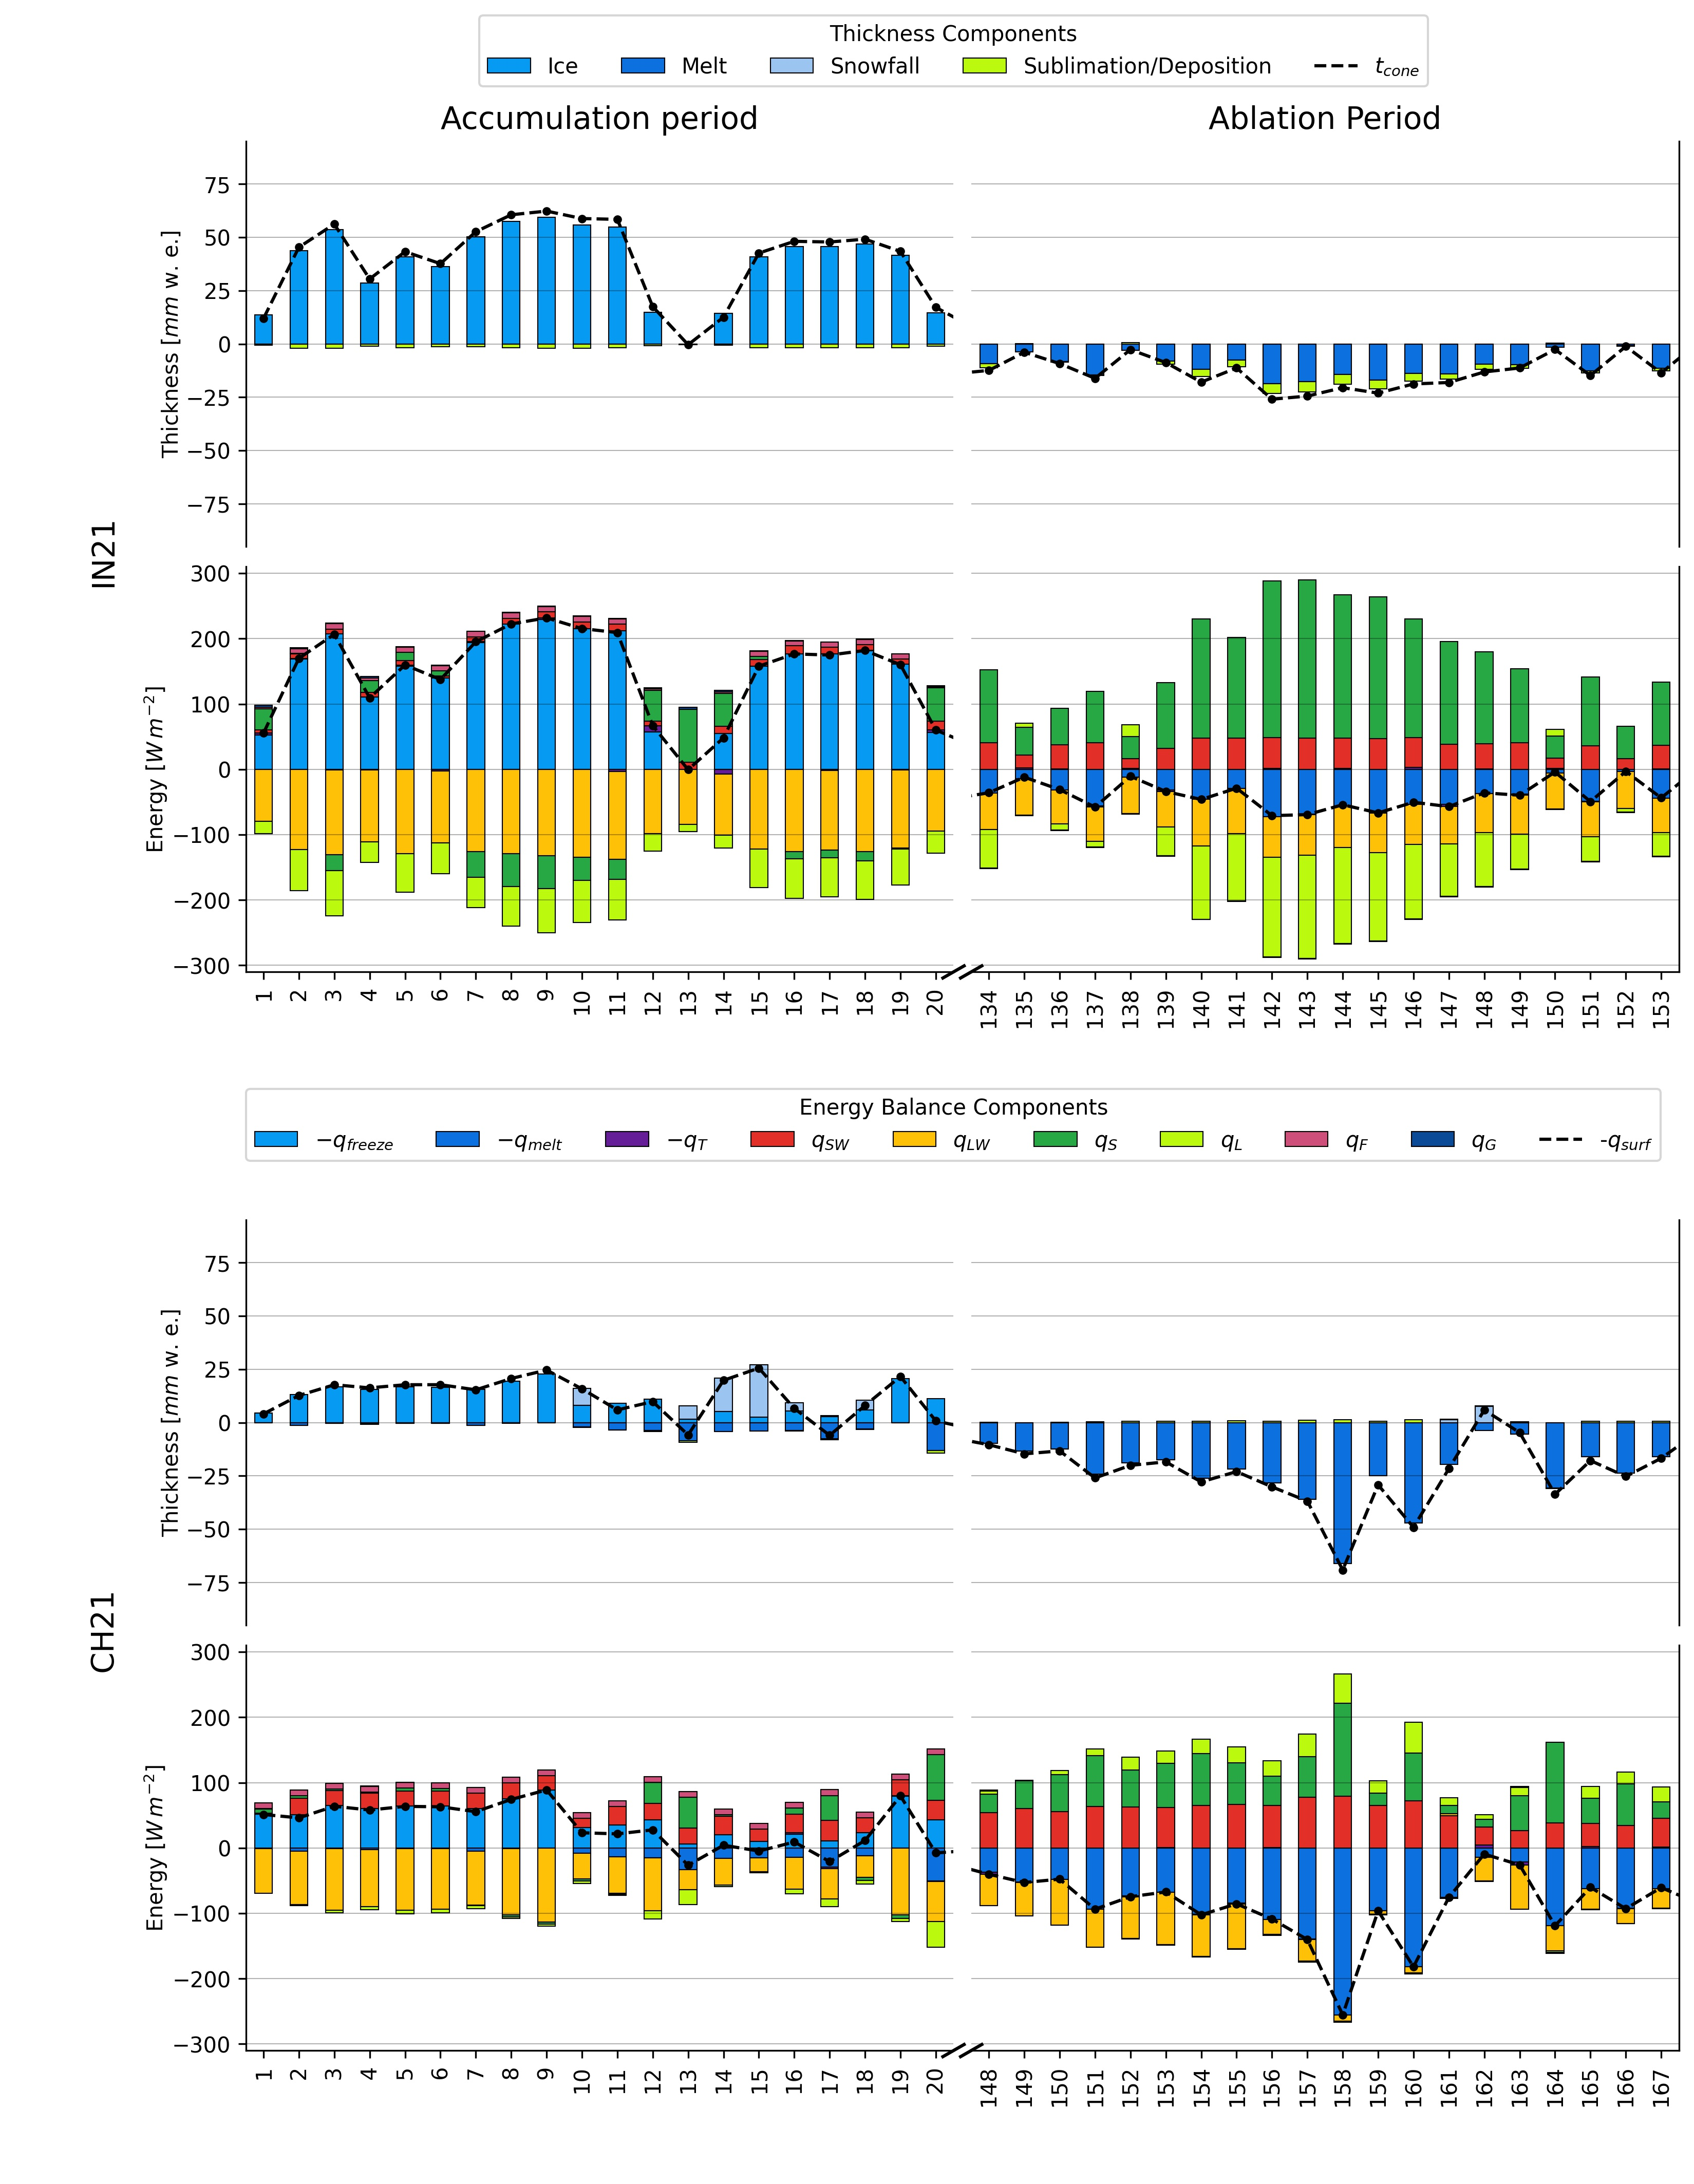
\includegraphics[width=\linewidth]{Figures/Figure_7.jpg} \end{center}
	\caption{Daily averages of thickness and energy balance components for the Indian and Swiss AIRs during the
		first 20 days of the accumulation and the last 20 days of the ablation period respectively.  } \label{fig:MEB}
\end{figure}

The longwave radiation flux had the highest energy turnover during the accumulation period for both the
locations. It increased and decreased the freezing and melting energy balance components during the accumulation
and ablation period respectively. However, its magnitude was much lower in the ablation period compared to the
accumulation period since the rising air temperature increased the incoming longwave radiation in the ablation
period. The magnitude of longwave radiation flux was much higher for the Indian site as its incoming longwave
radiation was strongly reduced due to its low cloudiness (see Table \ref{tab:Observations}).

Direct shortwave radiation was more than three times higher for the IN21 location due to its higher altitude and
lower latitude. However, the both the energy turnover and the magnitude of the shortwave radiation was lower for
the Indian site compared to the Swiss (see Table \ref{tab:turnover}). This was because the higher diffuse
shortwave radiation at the Swiss location was compensating for its lower direct shortwave radiation. Since the
IN21 site has mostly clear days, its diffuse shortwave radiation was very low (see Table
\ref{tab:Observations}). Moreover, less than 20 \% of the AIR surface area on average was exposed to direct
shortwave radiation flux for both the locations due to the area fraction $f_{cone}$. Temporal variation in the
$f_{cone}$ factor due to increasing solar elevation angle and decreasing AIR slope leads to higher shortwave
radiation in the ablation period compared to the accumulation period. Albedo, on the other hand, only varied
temporally for the Swiss location because there was no precipitation for the IN21 site.

\begin{table}
	\centering
	\caption{ Summary of the mass balance and AIR characteristics estimated at the end of the respective
  simulation duration}
	\label{tab:Results}
	\begin{tabular}{@{}|llllll|@{}}
		\toprule
		\textbf{}              & \textbf{Name}                   & \textbf{Symbol} & \textbf{IN21} & \textbf{CH21} &
		\textbf{Units}                                                                                                       \\ \midrule
		\multicolumn{1}{|l|}{\multirow{3}{*}{\rotatebox[origin=c]{90}{Input}}}
		                       & Fountain discharge              & $M_F$           & \num{2.9e6}   & \num{9.7e5}     & $kg$  \\
		\multicolumn{1}{|l|}{} & Snowfall                        & $M_{ppt}$       & 0             & \num{5.6e4}   & $kg$  \\
		\multicolumn{1}{|l|}{} & Deposition                      & $M_{dep}$       & \num{6.3e3}   & \num{4.1e3}     & $kg$  \\ \midrule
		\multicolumn{1}{|l|}{\multirow{4}{*}{\rotatebox[origin=c]{90}{Output}}}
		                       & Meltwater                       & $M_{water}$     & \num{2.4e5} & \num{2.3e5}   & $kg$  \\
		\multicolumn{1}{|l|}{} & Ice                             & $M_{ice}$       & \num{2.2e5} & \num{2.9e2}    & $kg$  \\
		\multicolumn{1}{|l|}{} & Sublimation                     & $M_{sub}$       & \num{4.8e4} & \num{5.2e3}     & $kg$  \\
		\multicolumn{1}{|l|}{} & Fountain wastewater             & $M_{waste}$    & \num{2.5e6} & \num{8.0e5}     & $kg$  \\ \midrule
		\multicolumn{1}{|l|}{\multirow{7}{*}{\rotatebox[origin=c]{90}{AIR}}}

		                       & Freezing rate                   & ${\Delta M_{freeze}}/{\Delta t}$    & $11 \pm 7$    & $1 \pm 2$     & $l/min$ \\
		\multicolumn{1}{|l|}{} & Melting rate                    & ${\Delta M_{melt}}/{\Delta t}$      & $1 \pm 4$     & $1 \pm 2$     & $l/min$ \\
		\multicolumn{1}{|l|}{} & Thickness change                & $j_{cone}$      & $3 \pm 25$    & $-4 \pm 27$   &
		$mm \, w.\,e.$                                                                                                       \\
		\multicolumn{1}{|l|}{} & Accumulation, Ablation period   &                 & $52, 102$     & $91,79$       & $days$  \\
		\multicolumn{1}{|l|}{} & Net Water Loss                  &                 & 81            & 77
		                       & \%                                                                                          \\
		\multicolumn{1}{|l|}{} & Maximum Ice Volume              &                 & 685           & 154           & $m^{3}$ \\
		\multicolumn{1}{|l|}{} & Surface Area                    & $A_{cone}$      & $350 \pm 38$  & $127 \pm 34$  & $m^{2}$ \\\midrule
		\multicolumn{1}{|l|}{\multirow{3}{*}{\rotatebox[origin=c]{90}{Model}}}
		                       & Surface layer thickness & $\Delta x$ & 65          & 45            &                $mm$  \\
		\multicolumn{1}{|l|}{} & RMSE with ice volume        &                 & 30            & 9            & $m^{3}$ \\
		\multicolumn{1}{|l|}{} & Correlation with ice volume &                 & 0.98          & 0.96          &
		N.A.                                                                                                                 \\\bottomrule
	\end{tabular}
\end{table}

Turbulent fluxes play a very important role in the energy balance. Sensible heat flux had the highest energy
turnover during the ablation period for both the locations. It decreased and increased the freezing and melting
energy balance components. The Indian location had much higher sensible heat due to higher wind speeds and
higher temperature gradient between the AIR surface and the atmosphere. The sensible heat contributes much more
to the energy turnover during ablation period than the latent heat flux due to rising air temperature. Latent
heat flux does not vary much in energy turnover between the accumulation and ablation periods. For the Indian
site, latent heat flux increased and decreased the freezing and melting energy since sublimation process was
favored throughout the simulation duration. But for the Swiss location, latent heat increased both the freezing
and the melting energy since sublimation and deposition process was favored during accumulation and ablation
period respectively.

The mass contribution of the sublimation/deposition process shown in Table \ref{tab:Results} was significantly
smaller than the energy flux contribution of this process since the heat of vaporization is around nine times
higher than the heat of fusion. The magnitude of the sublimation/deposition process was significantly different
for both the AIRs.  IN21 AIR lost 2 \% of its mass input to the sublimation process compared to the 1 \% mass
loss for the CH21 AIR (see Table \ref{tab:Results}). For the IN21 AIR, mass gain due to the deposition process
was an order of magnitude smaller than the mass loss due to the sublimation process. For the CH21 AIR, there was
no significant difference between the mass lost to sublimation and mass gained by deposition. This was expected
since glaciers near the IN21 location have been hypothesized to lose a significant amount of mass through
sublimation as suggested by \cite{azam_2018}.

Hence, for both locations, incoming longwave radiation and diffuse shortwave radiation have a control on the
thickness growth . Similarly, sublimation has a reducing effect on the thickness change. Particularly, the
Indian location had a much higher thickness growth because its incoming longwave radiation and diffuse shortwave
radiation during the accumulation period was much lower than that of the Swiss location due to lower mean winter
temperature and less cloudiness. The Indian location had a similar mean thickness decay compared to the Swiss
location because its latent fluxes were acting against the sensible heat fluxes using the sublimation process
during the ablation period unlike in the Swiss location, where deposition process was favoured during the
ablation period due to higher relative humidity and temperature.

The fountain had some influence on the energy fluxes through its water temperature, temperature forcing and
albedo forcing. However, this influence was insignificant compared to its influence on the surface area.  The
variance of this surface area was quite low in the accumulation period since the ice radius was initialised and
bounded by the spray radius. So the thickness growth was uniformly scaled to produce the corresponding ice
volume. The higher spray radius of the Indian fountain resulted in a higher maximum ice volume but this was
accompanied by an earlier expiry date. This was because a larger surface area increased both the freezing and
the melting rate.

\section{Discussion}

\subsection{Model limitations}
\subsubsection{Fountain quantification}

The model requires the fountain spray radius to be provided for defining the fountain. This is a significant
limitation since the model is very sensitive to the spray radius parameter. Moreover, $r_F$ is not only
determined by the fountain characteristics but also due to refreezing and melting events across the AIR
perimeter. Therefore, the same fountain may produce different spray radius under different weather conditions.

Contrary to our model assumptions, the parameters used to define the fountain were actually not independent. The
fountain height, fountain aperture diameter (both ignored in this analysis), discharge rate, water temperature
and spray radius were related through the trajectories of the water droplets. Particularly the temporal
variation of both the spray radius and the water temperature were completely ignored in the model. During the
IN21 experiment, snow formation was observed indicating that the fountain water droplets have the potential to
freeze before deposition on the AIR surface. Modelling such processes would require modelling the conduction,
convection and nucleation processes that all droplets undergo during their flight time. Therefore, a proper
quantification of the fountain is much more complex and requires a closer look at the correlation of the
fountain parameters amongst themselves and with the weather parameters. This will be investigated in a follow up
study, with this study focusing on the weather aspects of the model.

\subsubsection{Shape assumption}

The RMSE between the drone and the model estimates of the surface area for the IN21, CH21 and CH20 AIRs were 69
\%, 25 \% and 65 \% of the maximum area of the respective AIRs (see Table \ref{tab:uav}). There are two crude
assumptions that lead to such a large error namely, assuming a conical shape and assuming a constant radius
during the accumulation period.

Both these assumptions are a consequence of favoring the model simplicity over accuracy. One could, for example,
model the AIR shape assuming its cross section is a gaussian curve instead of a triangle.  But such
methodologies will involve inclusion of even more model parameters.

\subsection{Model sensitivity}

The model was found to be very sensitive to the surface layer thickness parameter. Theoretically, the parameter
selection for $\Delta x$ is based on the following two arguments: (a) the ice thickness $\Delta x$ should be
small enough to represent the surface temperature variations every model time step $\Delta t$ and (b) $\Delta x$
should be large enough for these temperature variations to not reach the bottom of the surface layer. But
practically, this parameter is also the only one compensating for the model shape assumption. This is
particularly true for the IN21 AIR where in reality two AIRs merged leading to a drastically different shape
evolution compared to our model. Therefore, $\Delta x$ was found to be an outlier in our global sensitivity
analysis. 

\subsection{Model calibration and validation}

The calibration process used has an inherent temporal and spatial bias due to the choice of when and how many
drone surveys were possible in each location. Among the 5 surveys of IN21 AIR used for calibration, most of them
were conducted around early March when the AIR volume was near its maximum whereas the 7 surveys of the CH21
location were more evenly spaced out in comparison (see Table \ref{tab:uav}). Moreover, the fountain spray
radius is also biased as a consequence leading to further model error. Depending on the number of drone surveys
in the accumulation vs the ablation period, $r_F$ could be over or underestimated. This could be one of the
reasons we observe a poor validation with the CH20 AIR since the spray radius is derived from just one drone
survey in the accumulation period.

\subsection{Favourable AIR locations}

Weather conditions play a significant role in making the Indian AIR larger and survive longer than the
Swiss AIR, namely, cloudiness, temperature and relative humidity. The lower cloudiness and mean winter
temperature of the Indian location significantly reduce the net radiation flux during the accumulation period, enabling a faster AIR thickness growth.  The lower humidity favours the sublimation over the deposition
process, thus decreasing the magnitude of net turbulent fluxes during the ablation period. This
results in a slower thickness decay .  Hence, for AIRs with similar fountain parameters, we expect locations
with lower cloudiness, lower mean winter temperature to augment freezing rates and locations with lower humidity
to dampen melting rates.

\subsection{Water losses of AIRs}

The net water losses of IN21 and CH21 AIR were $81\,\%$ and $77\,\%$ of the total mass input, respectively. The
high water losses were caused by the fountain wastewater in both the AIRs. Therefore, the AIR wastes water
mostly during the accumulation period. The freezing rate of the IN21 AIR was less than $20\, l/min$ for more than
90 \% of the accumulation period, meaning that the growth was not limited by the water supply rate but by the
freezing efficiency. The CH21 AIR freezing rate was able to reach the mean fountain discharge rate provided,
albeit for only 2 hours out of the 2155 hours of fountain runtime available. 

\subsection{Fountain optimization}

Water losses could have been reduced in two ways: (a) reducing the fountain runtime $t_F$ and (b) decreasing the
mean fountain discharge $d_F$. For the CH21 AIR, strategy (a) could have saved considerable wastewater as no
freezing was possible for 37 \% of the accumulation period. For the IN21 site, strategy (b) would have yielded
the least water loss as freezing rate was more than half the mean discharge rate for just two hours . However,
strategy (b) will also lead to a reduction in $r_F$ if it is not accompanied by a suitable change in the
fountain height and aperture diameter. So it can only be applied using the model if the corresponding fountain
parameters are better parameterised.

Practically though, both the strategies are difficult to apply. It is unrealistic to expect someone constantly
switching the fountain on and off under subzero conditions in accordance with strategy (a). Yes, strategy (b) is
comparatively easier but the minimum discharge rate is further constrained by the critical discharge rate below
which the pipeline will freeze. However, both the strategies can simultaneously be applied if the construction
process is completely automated via a system that regulates the discharge in accordance with the model freezing
estimates. Such a system can also drain the complete pipeline to prevent any pipeline freezing events. Since
none of these functions are energy intensive, this system can be deployed anywhere using a solar powered energy
source.

\section{Conclusions}

In this paper, we have developed a bulk energy and mass balance model to simulate AIR evolution using data from
field measurements in Gangles, India and Guttannen, Switzerland. The use of these datasets, in combination with
the novel model allowed for an accurate representation of the complex evolution typical of an AIR. The model was
calibrated and validated with ice volume and surface area observations obtained via drone surveys. We calculated
the water losses, freezing and melting rates for each of the three AIRs and explained their corresponding
magnitudes in terms of the influence of the location chosen and the fountain used. Our main conclusions are
summarized below:

\begin{itemize}
	\item The model was successful in reproducing the observed ice volume evolution with a correlation greater
	      than $0.96$ and an RMSE less than $18 \, \%$ of the maximum ice volume for all the AIRs.

	\item The ice volume achieved after the accumulation period was much higher for the Indian AIR compared to the
	      Swiss AIRs. The lower radiation fluxes of the Indian location favored a faster thickness growth rate and the
	      spray radius of the Indian fountain produced a higher surface area compared to the Swiss counterparts. Thus,
        the more than three times higher mean surface area and four times higher mean thickness growth rate
        during the two times shorter accumulation period of the Indian location result in a four times higher
        maximum ice volume of the Indian AIR compared to the Swiss.

	\item The ablation period of the Indian AIR was longer than the Swiss AIRs. However, the lower turbulent fluxes resulted in
	      a slower thickness decay rate on a larger surface area. This rendered the differences between the IN21 and CH21
	      melting rates negligible. Since the accumulation period produced much higher ice volumes, the Indian AIR was
	      able to last much longer than the Swiss AIRs.

	\item Water losses were high ($>75\,\%$) mostly due to fountain wastewater for all the AIRs. Vapour losses were
	      insignificant ($<4\,\%$) in comparison. However, significant improvement in water storage efficiency is possible
	      through optimization of fountain discharge rate.

  \item The Indian construction site produced long lasting AIRs with higher maximum ice volumes since it was
    colder, drier and less cloudy compared to the Swiss construction site. Thus, the AIR technology is ideally
    suited to serve as a water management strategy, especially in dry and cold mountain regions impacted by
    climate change induced water stress.

\end{itemize}

\section{Appendix}

\subsection{Ladakh icestupa 2014/15} \label{sec:ladakhloss}

A 20 $m$ tall icestupa \citep{iceheight} was built in Phyang village, Ladakh at an altitude of 3500 $m$ a.s.l.
Assuming a conical shape with a diameter of 20 $m$, the corresponding volume of this icestupa becomes 2093 $m^3$ or
1,920 $m^3$ w.e. The fountain sprayed water at a rate of $210\, l\,min^{-1}$ \citep{waterinput} from $21^{st}$
January \citep{waterstart} to at least until $5^{th}$ March 2015 \citep{waterend} (around 43 nights). Assuming
fountain spray was active for 8 hours each night, we estimate water consumption to be around 4,334 $m^3$. Thus,
during the accumulation period of the icestupa, roughly 56 \% of the water provided was wasted.  This icestupa
completely melted away on $6^{th}$ July 2015 \citep{iceends}.

\subsection{Drone data processing} \label{sec:uav}

\begin{figure}
	\begin{center}
		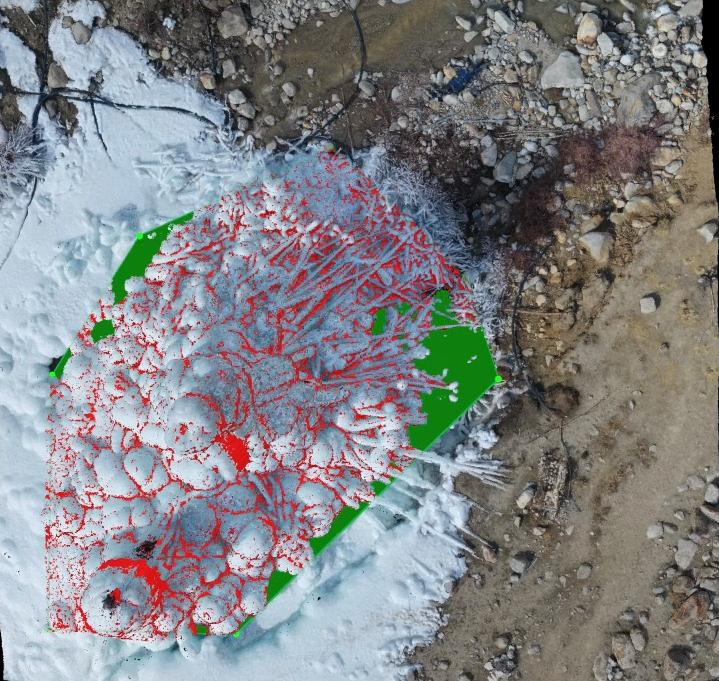
\includegraphics[width=10 cm]{Figures/gangles_DEM.jpg}
	\end{center}
	\caption{Digital elevation map of Indian AIR constructed from the drone survey on March 3, 2021. The green
		area represents the area bounded by the marked perimeter and the red area represents gaps in the point cloud
    generated by the software.
	}
	\label{fig:DEM}
\end{figure}

The drone flew automatically along a predefined flight course and took photographs at a certain time interval. The
position and altitude of the drone at the exposure stations, which were obtained by the built-in integrated
Position and Orientation System (POS, composed of global positioning system and inertial measurement units),
were recorded in the JPEG pictures. In this study, we adopted a three-step workflow as implemented in the
commercial software package Pix4Dmapper version 4.6.4 (\cite{Pix4D}). A short summary of this workflow is
described below:

(1) Initial processing: This process generates a sparse point cloud with the structure-from motion algorithm
(\cite{Turner_2012}). First, it searches for and matches key points in the photos that have certain overlapping
areas using a feature matching algorithm (e.g. the scale-invariant feature transform (SIFT) algorithm, which can
detect key points in photos with different views and illumination conditions; \cite{Lowe_2004}). Second, the
approximate locations and orientations of the camera at each exposure station are reconstructed with the internal
parameters (focal length, coordinates of the principal point of the photograph), and external parameters (i.e. POS
data). A sparse point cloud is created.

(2) Point cloud densification: In this step, the multi-view stereo technique is applied to achieve a higher point
cloud density than in the previous step (\cite{Furukawa_2010}; \cite{Molg_2017}). Thus, the spatial resolution of
the products can be increased, and an irregular network for the next step can be created (\cite{Kung_2011}).

(3) AIR delineation: Ice radius, area and volume are the three main final products. Perimeter was manually marked
on the point cloud by identifying the AIR boundary (see Fig. \ref{fig:DEM}). For the Indian location, we identified identical rock features
near the ice boundary to mark as vertices of this perimeter. For the Swiss AIR, no such feature was available due
to snowfall, so instead the perimeter was marked by identifying the ice and snow boundary.

There is temporal and spatial uncertainty associated with this process. Weather conditions influence the quality
of each drone survey variably. Moreover, since ice/snow surfaces do not have many identifiable features, few
feature points can be detected and matched in the vicinity of the AIR. Thus, we attach a high uncertainty of
$\pm 10 \%$ for all the AIR observations to accommodate for this.

\subsection{Sensitivity and uncertainty analysis} \label{sec:uncertainpy}
% \subsubsection{Uncertainty Quantification}
In this section, we summarise the theory behind the methods for uncertainty quantification and sensitivity
analysis used. For detailed explanation of this methodology, see \cite{uncertainpy_2018}.

\subsubsection{Problem definition}
Consider our model $U$ that depends on timestep $i$, has $d$ uncertain parameters $Q = [Q_1, Q_2, \dots, Q_d]$, and
gives output $V_{ice}$:

\begin{equation}
V_{ice} = U(i,Q)
\end{equation}

The output $V_{ice}$ can have any value within the output space and has an unknown probability density function
$\rho_{V_{ice}}$. The goal of our uncertainty quantification is to describe the unknown $\rho_{V_{ice}}$ through
statistical metrics.

We assume that all these parameters are statistically independent from each other and have a uniform probability
density function $\rho_{Q_j}$. The joint multivariate probability density function for the uncertain parameters
is then:

\begin{equation}
\rho_{Q} = \prod_{j = 1}^{d} \rho_{Q_j}
\end{equation}

As mentioned, the goal of an uncertainty quantification is to describe the unknown distribution of the model
output through statistical metrics. A useful metric is the $(100 \cdot x)$-th percentile $P_x$ of $V_{ice}$,
which defines a value below  which $100 \cdot x$ percent of the model outputs are located. We can combine two
percentiles to create a prediction interval $I_x$, which is a range of values within which a $100 \cdot x$
percentage of the outputs $V_{ice}$ occur: 

\begin{equation}
I_x = [P_{(x/2)}, P_{(1-x/2)}]
\end{equation}

The $90\,\%$ prediction interval, $I_{0.9}$, gives us the interval within which $90\,\%$ of the ice volume
outcomes occur, which also means that $5\,\%$ of the outcomes are above and $5\,\%$ are below this interval.

\subsubsection{Sensitivity analysis}

We use a variance-based sensitivity analysis and compute the commonly considered Sobol sensitivity indices
(Sobol, 1990). The Sobol sensitivity indices quantify how much of the variance in the model output each
uncertain parameter is responsible for. There are several types of Sobol indices. The first order Sobol
sensitivity index $S_j$ measures the direct effect each parameter has on the variance of the model. Higher order
Sobol indices give the sensitivity due to interactions between a parameter $Q_j$ and various other parameters.
The total Sobol sensitivity $S_{T_{j}}$ includes the sensitivity of both the first-order effects, as well as the
sensitivity due to interactions between a given parameter $Q_j$ and all combinations of the other
parameters. The sum of the total Sobol sensitivity indices is equal to or greater than one,
and is only equal to one if there are no interactions between the parameters. Our goal is to use sensitivity
analysis to fix parameters with low sensitivity, so it total-order Sobol indices are an appropriate metric.

\subsubsection{Polynomial Chaos Expansions}

A recent mathematical framework for efficient uncertainty quantification and sensitivity analysis is that of
polynomial chaos expansions (\cite{Xiu_2005}). This method calculates the same statistical metrics as the Monte
Carlo method but typically much faster.

The general idea behind polynomial chaos expansions is to approximate the model $U$ with a polynomial expansion
$\hat{U}$ : 

\begin{equation} U \approx \hat{U}(i, Q) = \sum_{n=0}^{N_p-1} c_n(i) \phi_n(Q) \end{equation}

where $\phi_n$ are polynomials, and $c_n$ are expansion coefficients. The number of expansion factors $N_p$ is
given by

\begin{equation}
  N_p = \binom{d+p}{p}
\end{equation}

where $p$ is the polynomial order. The polynomials $\phi_n(Q)$ are chosen so they are orthogonal with respect to the
probability density function $\phi_Q$.

The first and total-order indices can also be calculated directly from the polynomial chaos expansion. On the
other hand, the $90\, \%$ prediction interval ($I_{0.9}$) must be estimated by using $\hat{U}$ as a surrogate
model.

\section*{Conflict of Interest Statement} The authors declare that the research was conducted in the absence of
any commercial or financial relationships that could be construed as a potential conflict of interest.

\section*{Author Contributions} SB, MH, SW and FK designed the study.  SB developed the methodology with inputs
from MH.  MH, ML and JO reviewed the model algorithm and helped improve it. SB processed the drone data. JB helped
with model validation and uncertainty assessment. SB, MH, FK and SW participated in the fieldwork.  SB led the
writing of the paper and all co-authors contributed to it.

\section*{Funding} This work was supported and funded by the University of Fribourg and by the Swiss Government
Excellence Scholarship (SB). The associated fieldwork in India was supported by Himalayan Institute of
Alternatives and funded by the Swiss Polar Institute.

\section*{Acknowledgments} This work would not have been possible without the untiring efforts of the Swiss and
Indian icestupa construction teams through the winters of 2019, 2020 and 2021. We thank Mr. Adolf Kaeser and Mr.
Flavio Catillaz from Eispalast Schwarzsee (CH19); Daniel Beurki from the Guttannen Bewegt Association (CH20 and
CH21); Norboo Thinles, Nishant Tiku, Sourabh Maheshwari and the icestupa project team from HIAL (IN21).  We
would also like to thank Hanseuli Gubler for designing the Swiss AWS; Dr. Tom Matthews for designing the Indian
AWS; Michelle Stirnimann for conducting the CH20 drone surveys and Digmesa AG for subsidising their flowmeter
used in the experiment.  We would particularly like to thank Prof. Thomas Schuler and 4 anonymous reviewers who
gave us important inputs to improve the paper. We also thank Prof. Christian Hauck, Prof. Nanna B. Karlsson and
Dr. Andrew Tedstone for valuable suggestions that improved the manuscript.

\section*{Data Availability Statement} AIR timelapses (CH20, CH21) and results can be viewed interactively in
the web app.  The latest version of the web app and the model code  is available in GitHub
(\url{https://github.com/Gayashiva/air_model}, last access: 17 December 2021). The drone data can be obtained from
the authors upon request.

\bibliographystyle{frontiersinSCNS_ENG_HUMS} \bibliography{references}

\end{document}
